\documentclass[]{final_report}
\usepackage{graphicx}
\usepackage{hyperref}
\usepackage{listings}
\usepackage{graphicx}
\usepackage[utf8]{inputenc}
\usepackage{subcaption}
\usepackage[backend=biber,style=numeric,sortcites,natbib=true,sorting=none]{biblatex}
\addbibresource{refs.bib}


%%%%%%%%%%%%%%%%%%%%%%
%%% Input project details
\def\studentname{James Arnott}
\def\reportyear{2023}
\def\projecttitle{Comparison of Image Classification Models with Transfer Learning}
\def\supervisorname{Li Zhang}
\def\degree{BSc (Hons) in Computer Science}
\def\fullOrHalfUnit{Full Unit} % indicate if you are doing the project as a Full Unit or Half Unit
\def\finalOrInterim{Final Report} % indicate if this document is your Final Report or Interim Report

\begin{document}

\maketitle

%%%%%%%%%%%%%%%%%%%%%%
%%% Declaration

\chapter*{Declaration}

This report has been prepared on the basis of my own work. Where other published and unpublished source materials have been used, these have been acknowledged.

\vskip3em

Word Count: XXXX % TODO: Word count

\vskip3em

Student Name: \studentname

\vskip3em

Date of Submission: \today

\vskip3em

Video Link: % TODO: video

\vskip3em

Signature:
\begin{figure}[ht!]
  
\includegraphics[width=50mm]{images/signature.jpg}
\end{figure}

\newpage

\tableofcontents\pdfbookmark[0]{Table of Contents}{toc}\newpage

\begin{abstract}

Transfer learning is an effective and widely used method for training deep learning models by utilizing pre-trained models to extract features from a dataset and training a new model on these features. This project report compares the performance of several image classification models, including Mobilenetv3, InceptionV3, ResNet, VGG, EfficientNet and Xception, when applied to transfer learning. The models are evaluated on a dataset consisting of MRI scans of Alzheimer's patients and images of skin cancer, which highlights the importance of accurate diagnosis and classification in the medical field. The project aims to achieve the highest accuracy in classification by exploring various optimization techniques for neural networks. By comparing these models, this study provides valuable insights into their applicability and potential improvements for similar transfer learning tasks in the future.% TODO: add a breif summary of the results

The Web-UI URL is here\cite{Hosted-UI} on GitHub Pages.
\end{abstract}

%%%%%%%%%%%%%%%%%%%%%%
%%% Project Spec
% TODO: Software Engineering, show use of GIT and LaTeX, do uml? Show TDD with jupyter notebooks?
% TODO: Summary of completed work
% TODO: Ensure the models being compared are right

\chapter*{Project Specification}

Aims: To implement and compare on benchmark data sets various machine learning algorithms
Background: Machine learning allows us to write computer programs to solve many complex problems: instead of solving a problem directly, the program can learn to solve a class of problems given a training set produced by a teacher. This project will involve implementing a range of machine learning algorithms, from the simplest to sophisticated, and studying their empirical performance using methods such as cross-validation and ROC analysis. In this project you will learn valuable skills prized by employers using data mining.
Early Deliverables

\begin{itemize}
  \item You will implement simple machine learning algorithms such as nearest neighbours and decision trees.
  \item They will be tested using simple artificial data sets.
  \item Report: a description of 1-nearest neighbour and k-nearest neighbours algorithms, with different strategies for breaking the ties;
  \item Report: a description of decision trees using different measures of uniformity.
\end{itemize}

\section*{Final Deliverables}
\begin{itemize}
  \item May include nearest neighbours using kernels and multi-class support vector machines.
  \item The algorithms will be studied empirically on benchmark data sets such as those available from the UCI data repository and the Delve repository.
  \item For many of these data set judicious preprocessing (including normalisation of attributes or examples) will be essential.
  \item The performance of all algorithms will be explored using a hold-out test set and cross-validation.
  \item The overall program will have a full object-oriented design, with a full implementation life cycle using modern software engineering principles.
  \item Ideally, it will have a graphical user interface.
  \item The report will describe: the theory behind the algorithms.
  \item The report will describe: the implementation issues necessary to apply the theory.
  \item The report will describe: the software engineering process involved in generating your software.
  \item The report will describe: computational experiments with different data sets and parameters.
\end{itemize}

\section*{Suggested Extensions}
\begin{itemize}
  \item Modifications of known algorithms.
  \item Dealing with machine learning problems with asymmetrical errors (such as spam detection) and ROC analysis.
  \item Nontrivial adaptations of known algorithms to applications in a specific area, such as medical diagnosis or option pricing.
  \item Exploring the cross-validation procedure, in particular the leave-one out procedure. What is the optional number of folds?
  \item Comparative study of different strategies of reducing multi-class classifiers to binary classifiers (such as one-against-one, one-against-the-rest, coding-based).
\end{itemize}

\section*{Reading}
\begin{itemize}
  \item Trevor Hastie, Robert Tibshirani, and Jerome Friedman. The Elements of Statistical Learning. Second edition. Springer, New York, 2009.
  \item Tom M. Mitchell. Machine Learning. McGrow-Hill, New York, 1997.
  \item Vladimir N. Vapnik. The Nature of Statistical Learning Theory. Second edition. Springer, New York, 2000.
  \item Vladimir N. Vapnik. Statistical Learning Theory. Wiley, New York, 1998.
  \item Seth Hettich and Steven D. Bay. The UCI KDD Archive. University of California, Department of Information and Computer Science, Irvine, CA, 1999, http://kdd.ics.uci.edu.
  \item Delve archive. http://www.cs.toronto.edu/~delve.
\end{itemize}

\section*{Addendum}
As I was not keen on doing the pre-assigned generic project, I had asked for permission to do a project of my own choosing.
I was given permission to do so, and I chose to do a project on comparison of image classification models using transfer learning.
I chose this project as I was interested in transfer learning as I had used it in a previous project and wanted to learn more about it
and it seemed far more interesting than the generic project and I believe this is generally a more applicable problem to solve in the real world.

\chapter{Rationale}

\section{Introduction}

My project is about the comparison of image classification models with transfer learning.
In this report I shall cover the background of transfer learning, the models I have chosen to compare, the datasets I have chosen to use, the pre the results of my experiments and the conclusions I have drawn from them.

The importance of transfer learning cannot be overstated, it makes training models for anyone with a computer and an internet connection possible, It opens up possibilities for people who would otherwise not be able to train models as far fewer data points and computing power is required and where properly applied, they can be more accurate than models trained from scratch.

In this project, I'm planning to learn about transfer learning and comparing the different models and also going over other methods of classification such as SVMs and KNNs. I will then preprocess the dataset images and train the models on the dataset and compare the results. I will then attempt to optimise the models, find out what issues they have and try to fix them to get the best results possible.

I'll also make a web based GUI for the project, so that anyone can use it to classify images of their own. I plan on using python based libraries such as keras and flask, which will communicate with a backend server. I also plan to use and test the viability of tensorflowJS\cite{smilkov2019tensorflowjs} to make the model run in the browser, which would allow anyone to use the model locally, without having to send their images to a server, which would avoid all privacy issues and potential legal issues.

This will be a learning experience for me, as I have not done any machine learning work before, and I will get to learn about different machine learning techniques and experiment with cutting edge technology that is being used in the real world.



\section{Objectives}


The main objectives of this project are:

% Begin List
\begin{itemize}
  \item Understand the core principles of transfer learning, its benefits, and its applications in image classification.
  \item Research appropriate image classification models for comparison, as well as documenting alternative classification techniques (such as SVMs and KNNs).
  \item Identify suitable datasets for training and evaluating the models.
  \item Preprocess dataset images and explore data augmentation techniques if necessary.
  \item Train the selected models (with transfer learning) and compare their performance.
  \item Optimize the models, identify their limitations, and implement strategies to improve their performance.
  \item Develop a user-friendly web-based GUI for image classification using the trained models.
  \item Assess the feasibility and benefits of using TensorFlow.js to enable client-side execution of the models.
\end{itemize}

\section{Background}
Alzheimer's disease is a neurodegenerative disease that affects the brain. It is the most common cause of dementia, and 1 in 3 people born in the UK this year will develop dementia in their lifetime.\cite{DementiaStatistics}

The symptoms of Alzheimer's disease are memory loss, confusion, mood swings, and difficulty with everyday tasks, it can also eventually lead to death, however the slow progression disease causes many prople to live with it for years and slowly lose their independence, and forget who they are.

There have recently been developments in drug discovery and development that have been able to slow the progression of AD, but are only effective in the early stages of the disease, and are not able to reverse the damage that has already been done. This means that early diagnosis is essential to ensure that the drugs are as effective as possible.\cite{Van_Dyck2022-pt}

Transfer learning can be a useful tool to create predictions of the progression of AD, as it can be used to train models on a smaller dataset than would otherwise be required, as MRI scans are expensive and time consuming to obtain.

\chapter{Neural Networks}
\begin{figure}[ht!]
  \centering
  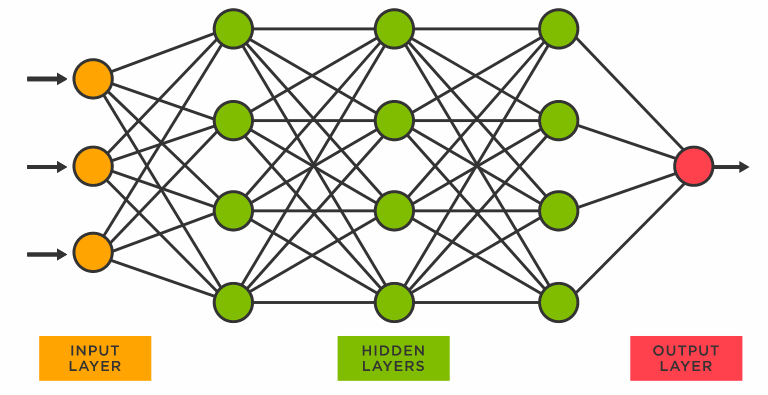
\includegraphics[width=100mm]{images/NeuralNetwork.png}
  \caption{A diagram of a neural network \cite{NeuralNetworkDiagram}}
\end{figure}

\section{What is a Neural Network}
A neural network is a machine learning model that is inspired by the way the human brain works.
It is made up of a series of layers, each layer is made up of a number of neurons.
Each neuron is connected to every neuron in the next layer (in fully connected layers, they're not all like that however), and each connection has a weight associated with it.
The weights are used to determine how much each neuron in the next layer is affected by the current neuron.
The weights are updated during training, and the process of updating the weights is known as backpropagation.

Convolutional Neural Networks or CNNs are the main time of neural networks I will be using for this project, as they are currently the best performing type of neural network for image classification.

Deep learning is a type of machine learning that uses neural networks, but with many more layers than traditional neural networks, and many of the models I will be using would be considered to be deep learning models.

\section{Why use a Neural Network}
The use of neural networks has increased dramatically in recent years, and they are now used in a variety of different applications.
The reason for this is that they are very good at learning complex patterns in data, and they are able to learn
these patterns without being explicitly programmed to do so. This saves a lot of time and effort when compared to other machine learning techniques.

They are far more flexible than many of the traditional strategies for image classification, due to the fact they can adapt to new data and are
resilient to noise in the data or changes such as lighting or rotation.

\pagebreak
\section{What are the alternatives to Neural Networks in Image Classification}

This is not an exhaustive list for image classification, but it is a list of some of the most common alternatives to neural networks
that produce the best results.

\subsection{Support Vector Machines}
There are a number of different alternatives to neural networks, one common alternative is Support Vector Machines.
Support Vector Machines are a type of supervised machine learning model that can be used for both classification and regression.
They work by finding a hyperplane that separates the data into different classes, and then classifying new data based on which side of the hyperplane it is on.
They are very good at classifying data that is linearly separable, otherwise they are not as good, and they are also very typically sensitive to noise in the data, if they are not properly tuned, and this can take a long time to do. Another drawbacks of SVMs is that they can be less accurate with data that has a high dimensionality.

In one study using SVMs to classify Alzheimer's patients, the researchers managed to get an accuracy of 62.64\% using MRI scans of the brain.
They managed to get between 83\% and 90\% accuracy when using SVMs with clinical parameters, however combining the two methods in this study did not improve the accuracy. \cite{10.3389/fneur.2021.640696}

Random Forests and Decision Trees can also be used for image classification. They are more interpretable compared to neural networks and can be efficient when dealing with smaller datasets. They are however not as accurate as neural networks generally, so they are not as commonly used for image classification.

\subsection{Content Based Image Retrieval}
Content Based Image Retrieval (CBIR) is a type of image retrieval system that uses the actual content of an image as the basis for retrieving similar
images from a large database. It works by extracting the features from the image and then using those features to compare to other images in the database.
The features are usually based on a combination of color, texture, shape, and other attributes. The system then produces a list of images that are similar
to the one used for the search query. CBIR systems are particularly useful for searching for images that can't be easily described using traditional keywords.

CBIR can be used to identify images that are not in the database by analyzing the content of the images.
By extracting features from the image such as color, texture, and shape, CBIR can be used to compare the
content of the query image with the content of the images in the database. It can then return images that are
similar in content to the query image even if they are not present in the database.

For example, if the target image was a blue sky with white clouds, then the algorithm would return
images that had similar features such as a blue sky and white clouds to the target image.

Although this method of image classification would not seem to be very useful for classifying images of Alzheimer's patients,
a study was done using this method to classify Alzheimer's patients, and they had managed to get an accuracy of 87\% using MRI scans\cite{5972513}
and getting feedback from the physicians who were treating the patients.

For classifying images of different flowers, for example, it could also be very useful, as it would allow the user to search for images of a specific flower.
This could help identify flowers by recognizing the different characteristics of each flower, such as the shape of the petals,
the color of the petals, and the overall structure of the flower.

\section{The Different Optimisers}

In deep learning, optimisers are algorithms used to adjust the parameters of a model in order to minimise a loss function. Optimisers are used to improve the accuracy of a model by reducing the error rate. Common optimisers used in deep learning include Stochastic Gradient Descent (SGD), Adaptive Moment Estimation (Adam), and Root Mean Square Propagation (RMSProp). There are many optimisers that can be used to train a model, and the one that is used depends on the type of problem that is being solved.

The impact using different optimisers can have is dependent on the type of problem being solved. For example, SGD is often used for linear regression problems, while Adam is better suited for deep learning problems. Additionally, the choice of optimiser can also affect the speed of convergence and the accuracy of the model. However, there isn't always a one-size-fits-all solution, and it is often necessary to experiment with different optimiser and their hyperparameters to find the best fit for a specific problem.

\begin{figure}[h]
  \centering
  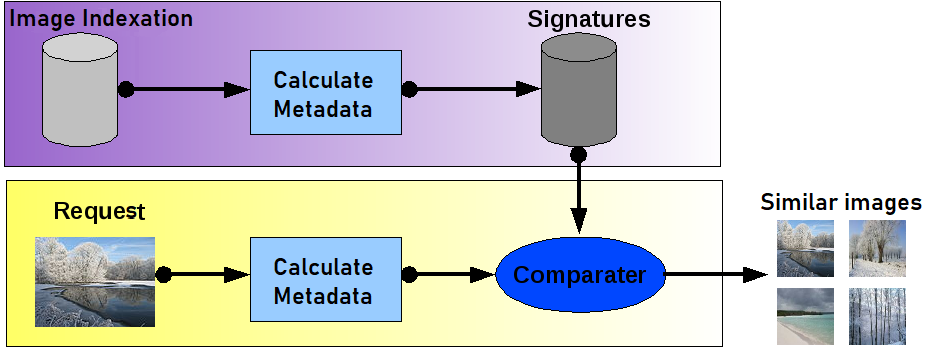
\includegraphics[width=0.7\textwidth]{images/Principe_cbir.png}
  \caption{A diagram of Content Based Image Retrieval \cite{ContentBasedImageRetrieval}}
\end{figure}

\section{Classification Vs Regression}

Classification is a type of supervised machine learning model that is used to predict the class of a given data point. It is used to predict the class of the given data, whereas regression is used to predict the value of a given data point. For example, classification would be best suited to classifying images for dogs or cats, whereas regression would be best suited to predicting the price of a house. Regression in machine learning is also a type of supervised learning model that is used to predict the value of a given data point.

Alzheimer's disease is not a binary classification problem, as it is not a case of either having Alzheimer's or not having Alzheimer's, it is more of a spectrum of different stages of the disease. The OASIS-1 dataset contains a CDR score for each patient, which is a measure of the severity of the disease. This means that the problem is more of a regression problem, as it is trying to predict the severity of the disease, rather than trying to classify the patient as having Alzheimer's or not, however as there are only 4 different scores in the dataset, classification may be more suited to this problem, for this specific dataset. There could however be an argument made that this could be a multi-class classification task, as the model could try and just estimate the most likely scores for the patient, rather than trying to predict the exact score, which could be more useful to a doctor.

In the case of the skin cancer dataset, the problem is a binary classification problem, as the dataset only contains images of either benign or malignant skin cancer. This means that the given images are either of a benign or malignant skin cancer, and the model is trying to predict which one it is.

\section{What is a Convolutional Neural Network}
A convolutional neural network (CNN) is a type of neural network that is used for image classification. It is made up of a series of convolutional layers, pooling layers, and fully connected layers. The convolutional layers are used to extract features from the image, and the pooling layers are used to reduce the size of the image. The fully connected layers are used to classify the image. They are often much more efficient than other types of neural networks, and are commonly used for image classification. CNNs are more suited to multi-dimentional data, such as images, as they are able to extract features from the image and then use those features to classify the image.

Dropout layers are used to reduce overfitting in the model. Overfitting is when the model is too specific to the training data, and is unable to generalise to new data. This can be a problem when the model is used to classify images that it has never seen before, such as the validation sets I am using for this project. Dropout layers randomly ignore nodes during training, which leads to the model being less specific to the training data, and therefore being able to generalise to new data better.

CNNs are not just restricted to image classification, they can also be used for other types of classification problems. For example, they can be used to classify text and audio too (amongst other data).

\section{Types Of Layers}

% Listing the different types of layers
\begin{itemize}
  \item Convolutional Layer: This layer extracts features from an input image and creates a feature map.

  \item  Pooling Layer: This layer reduces the dimensionality of a feature map while preserving its most important features.

  \item  Dropout Layer: This layer randomly ignores nodes during training to reduce overfitting.

  \item  Fully Connected Layer: This layer connects all the neurons of the previous layer to every neuron in the next layer. It helps in mapping input to output.
\end{itemize}

% Talk about the different types of layers specifically
% Include a diagram of a CNN

\section{Using an LSTM for classification with MRI scans}
An LSTM (Long Short Term Memory) network is a type of recurrent neural network that is used for time series prediction, it is typically not used with transfer learning as it is not as efficient as other types of neural networks. The specific LSTM structure allows for multiple MRI scans to be used as input to the model, and the model, so it would be able to classify the Alzheimer's CDR score more accurately, as it could take into account more scans, using the raw scan information, instead of the pre-processed data that I would otherwise have to use with regular CNN model that I could use with transfer learning.

This would be interesting to explore as it would be a new way of using an LSTM model, and it would be more space efficient, than having a neural network take the 3D MRI scans as input, as it would be able to take in the 2D slices of the MRI scans as input, and use the LSTM model to process the data. 
This technique could potentially lead to improved accuracy in Alzheimer's disease diagnosis and a better understanding of the progression of the condition.

\section{What transfer learning is}
Transfer learning is a prevalent and efficient method for training deep learning models. There are numerous ways to implement transfer learning, and this discussion aims to compare the performance of various methods with different pre-trained models.

The applications for transfer learning are extensive, as it is a frequently used method to train deep learning models. It is primarily due to the method's efficiency in training models, as most of the work is performed by the pre-trained model. This model is employed to extract features from the dataset, followed by training a new model on top of the extracted features. Typically, the pre-trained model is frozen, so it does not change during training; only the new model is trained.

Once the new model is trained on top, a process called fine-tuning can further enhance the model's performance. Fine-tuning involves training the new model on the dataset but with a lower learning rate than the initial training. At this stage, the model is usually unfrozen, allowing the pre-trained model to be trained as well, leading to improved overall performance.

It is possible to use a pre-trained model as a feature extractor, such as an SVM or a logistic regression model, instead of just neural networks.

\chapter{The Datasets I will be using}
The dataset I have chosen to primarily use for this project is the OASIS-1\cite{OASIS} dataset.
This dataset contains 416 patients, ageing from 18 to 96 years old. It is primarily composed of patients without Alzheimer's disease.

I have also chosen to include another dataset which should be easier to classify it's used in the Intelligent skin cancer diagnosis using improved particle swarm optimization and deep learning models\cite{TAN2019105725}.
It's a combination of 2 datasets, the Edinburgh Research and Innovation (Dermofit)\cite{Ballerini2013}, and the Dermatology Service of Hospital Pedro Hispano\cite{6610779}. There are 484 images in the dataset, with 2 different classes, benign (270) and malignant (214). All the images are 200x200 pixels, with 3 channels (RGB), which is not optimal as they require upscaling to be used with the models I will be using for transfer learning.

In the paper from the dataset creators, they used KNN, SVM and a CNN model to classify the images in the dataset.
With the optimal hyperparameters, they achieved an accuracy of 99.54\% using the SVM and RCPSO which stands for Real-Coded Particle Swarm Optimization, this is a nature-inspired optimization technique used to search for the best solution in a given problem space, which was used for optimising the hyperparameters of the SVM model.

\section{The Contents of OASIS-1}
This information is from the fact sheet, associated with the dataset. \cite{OASISFactSheet}
The OASIS-1 dataset contains a few different associated parameters, as listed here from the CSV:

`ID,M/F,Hand,Age,Educ,SES,MMSE,CDR,eTIV,nWBV,ASF,Delay`

\begin{itemize}
  \item ID: The ID of the patient
  \item `M/F`: The gender of the patient
  \item `Hand`: The primary hand of the patient
  \item `Age`: The age of the patient
  \item `Educ`: The education level of the patient 1: less than high school grad., 2:High school grad., 3: some college, 4: college grad., 5: beyond college
  \item `SES`: The socioeconomic status of the patient
  \item `MMSE`: The Mini-Mental State Examination score of the patient
  \item `CDR`: The Clinical Dementia Rating score of the patient
  \item `eTIV`: The Estimated Total Intracranial Volume of the patient
  \item `nWBV`: The normalized whole brain volume of the patient
  \item `ASF`: The Atlas Scaling Factor of the patient
\end{itemize}

The augmentations I can use for this dataset cannot be as extensive as the skin cancer dataset, as the scans are pretty consistent in size and shape, along with being in greyscale, so I will only be using the following augmentations:
\begin{itemize}
  \item Random horizontal flipping
  \item Random vertical flipping
  \item Random rotation (20 degrees)
  \item Random zoom
\end{itemize}

\section{The Contents of the Skin Cancer Dataset}

The skin cancer dataset contains 2 different classes, benign and malignant, and 484 images in total.
This is all the information that is available about the dataset, as it is not a publicly available dataset, this requires me to augment the data as much as possible to get good results.

The augmentations I will be using are:
\begin{itemize}
  \item Random horizontal flipping
  \item Random vertical flipping
  \item Random rotation
  \item Random zoom (359 degrees)
  \item Random brightness
  \item Random offset
\end{itemize}

Augmentations on the skin cancer dataset would represent more of a real-world scenario as opposed to the OASIS-1 dataset, as the scans are all in the same orientation, whereas the oritentation of the images in the skin cancer dataset could practically be at any orientation and still be valid.

\chapter{The Different Models That Are Being Compared}

All the pre-trained models are from the Keras library\cite{Keras} and were trained on the ImageNet dataset\cite{ImageNet}.

\section{Mobilenetv3}

As described in the "Searching for Mobilenetv3" paper\cite{DBLP:journals/corr/abs-1905-02244}, this model is designed for mobile devices, and is a successor to the Mobilenetv2 model.
It is a comparatively small model as it is optimised for mobile devices, and is also very fast.

The resulting models from this paper are:
\begin{itemize}
  \item Mobilenetv3-Large
  \item Mobilenetv3-Small
\end{itemize}

The idea to have a large and small model is to specialise the model for different use cases and different hardware, increasing the speed or accuracy of the model.
The large model is designed for high accuracy, and the small model is designed for high speed, there may also be cases where the smaller model is the only viable option due to hardware constraints.

% insert the image of the mobilenetv3 structure
\begin{figure}[ht!]
  \centering
  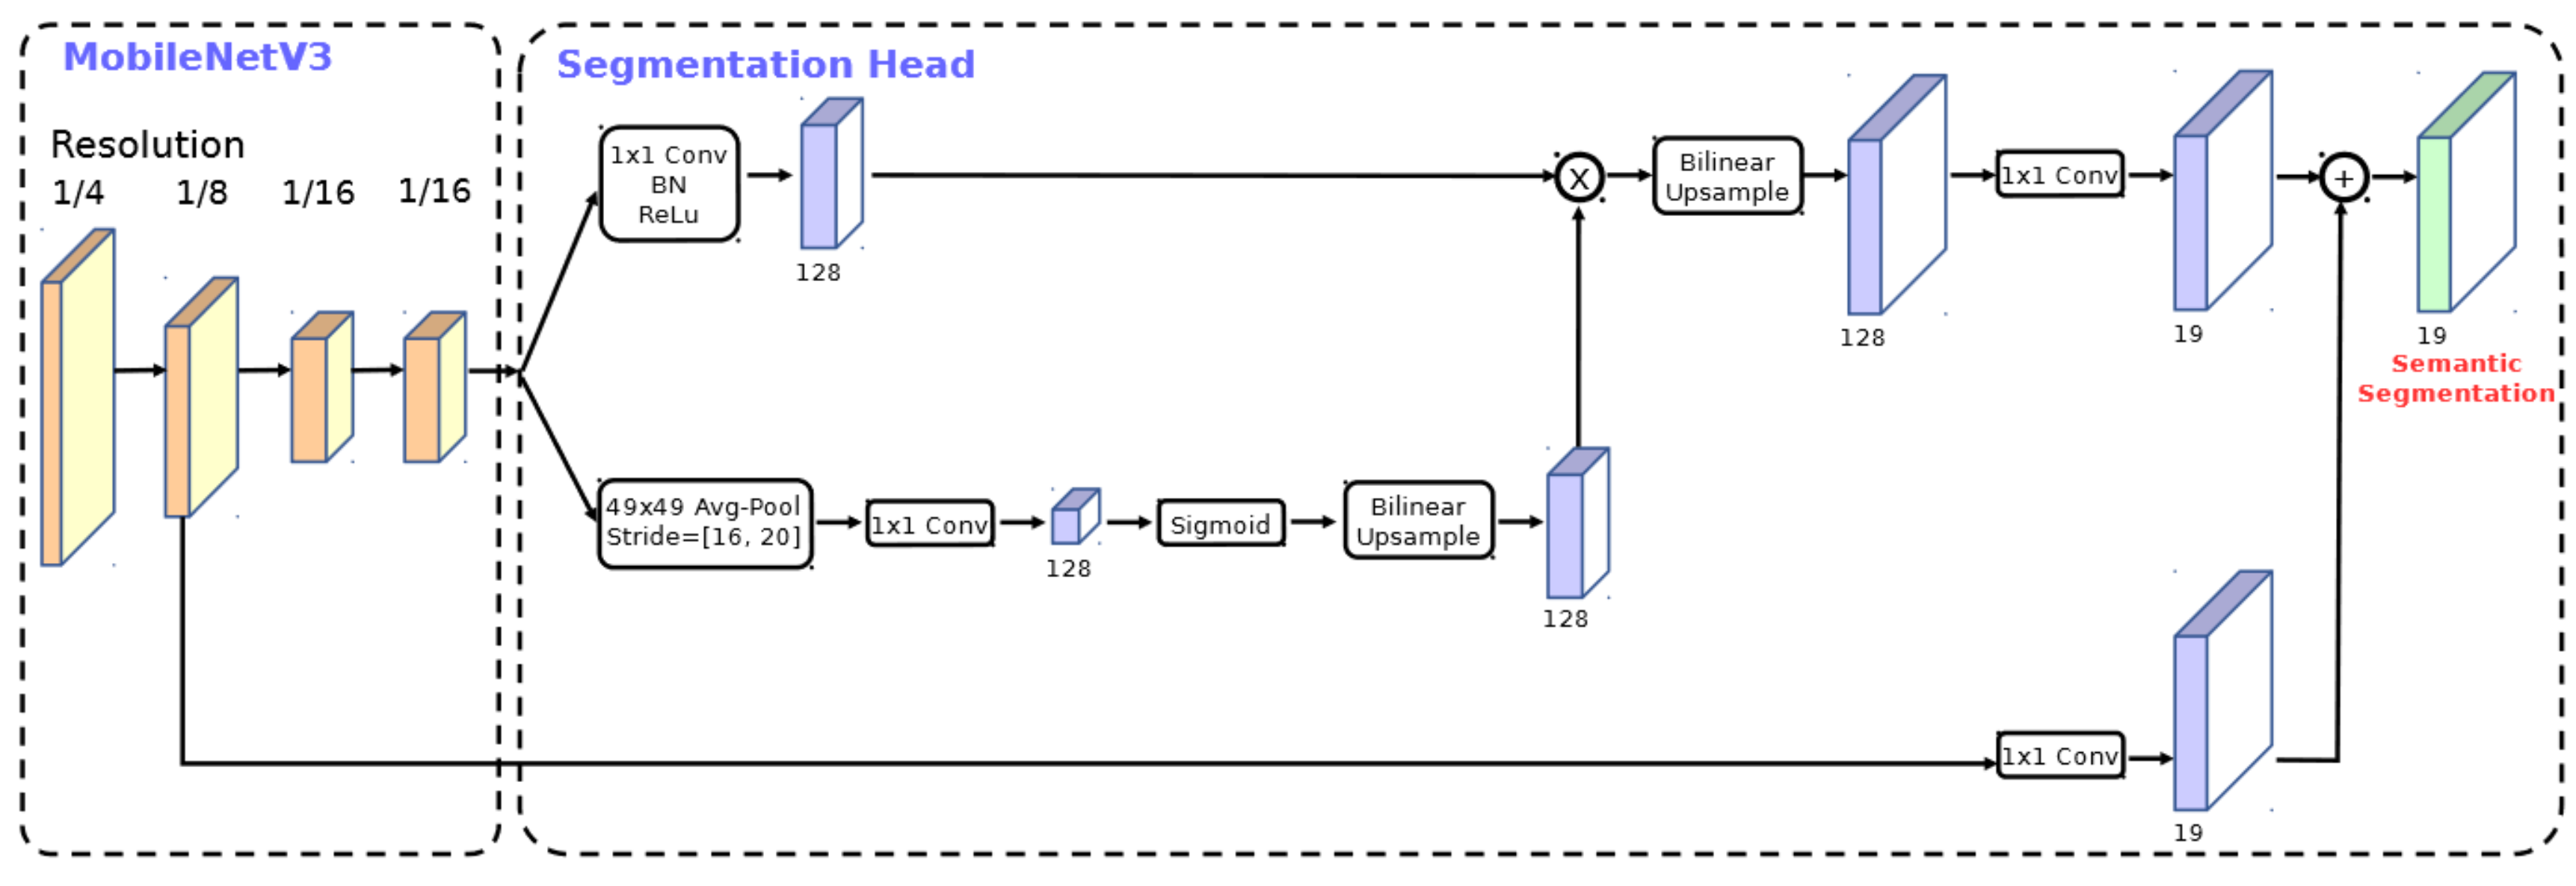
\includegraphics[width=0.8\textwidth]{images/MobileNetv3-structure.png}
  \caption{The proposed segmentation head for MobileNetV3\cite{DBLP:journals/corr/abs-1905-02244}}
  \label{fig:mobilenetv3-segmentation}
\end{figure}

\begin{figure}[ht!]
  \centering
  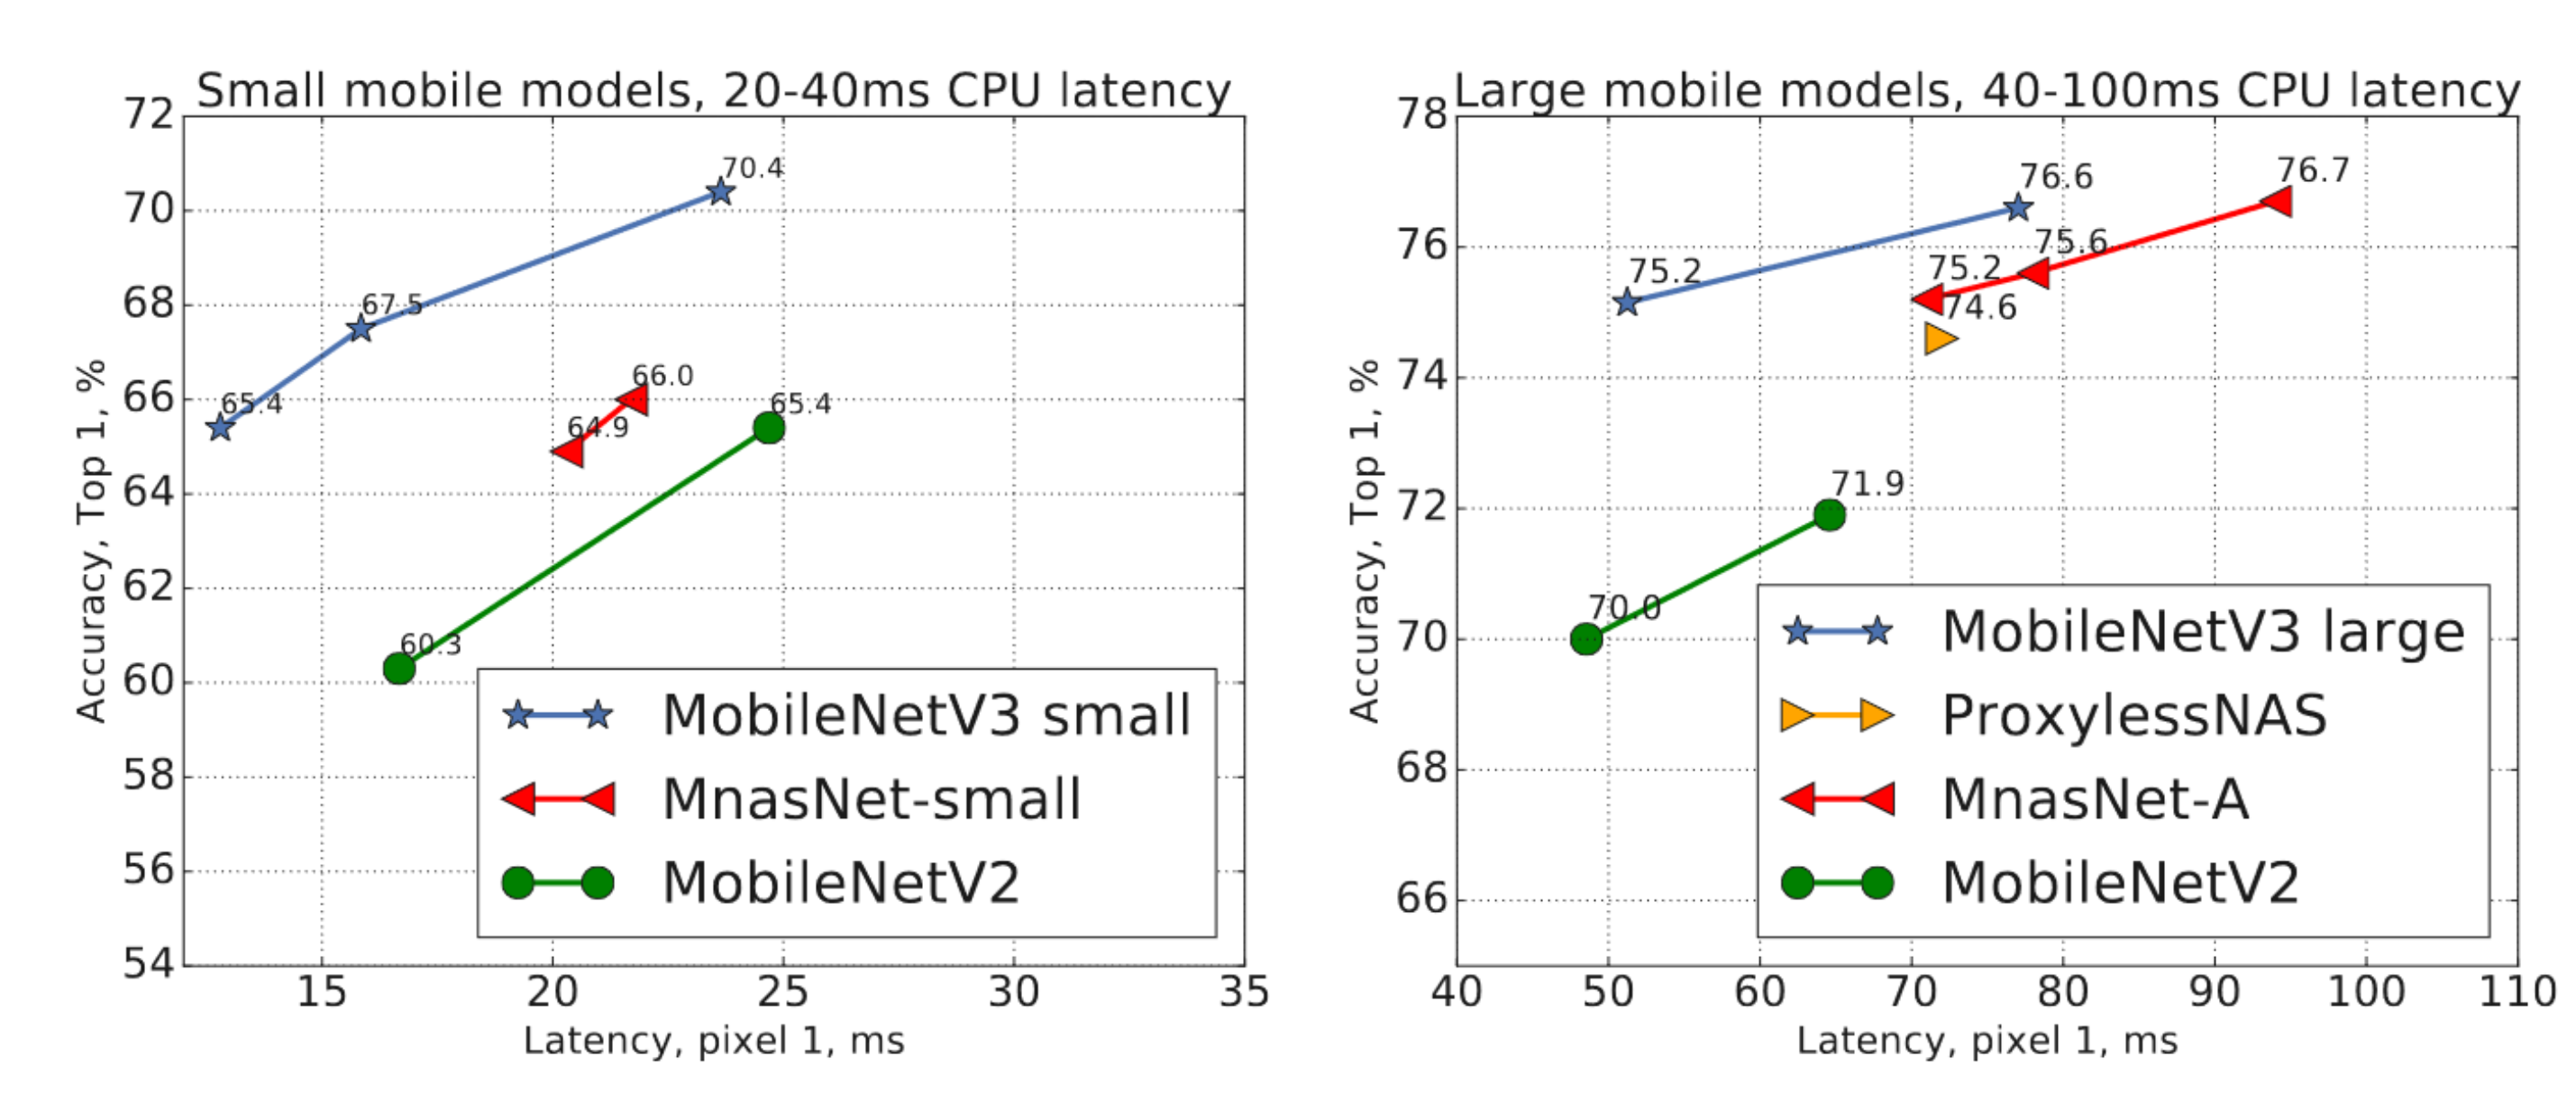
\includegraphics[width=0.8\textwidth]{images/mobilenet-comparison.png}
  \caption{A comparison of latency and accuracy\cite{DBLP:journals/corr/abs-1905-02244}}
  \label{fig:mobilenetv3-comparison}
\end{figure}


% TODO: Add the top performers from here https://paperswithcode.com/sota/image-classification-on-imagenet?metric=Top%205%20Accuracy&dimension=Number%20of%20params

\section{InceptionV3}
InceptionV3\cite{DBLP:journals/corr/SzegedyVISW15}, it's one of the most popular models for image classification as it is comparatively fast and accurate.
It's feature extraction capabilities are much more accurate than traditional methods such as hand-crafted feature extraction.
It is a deep learning model that uses a combination of convolutional layers, pooling layers, and fully-connected layers.
It uses auxiliary classifiers, these are additional classifiers used in a neural network to predict the output of the main classifier. Auxiliary classifiers are used to improve the accuracy of the main classifier by providing additional input data.
They can also help to reduce the amount of overfitting that can occur when using a single classifier.

\section{ResNet}
Resnet\cite{DBLP:journals/corr/HeZRS15} is another popular model, ResNet101 is the largest model that is being compared and different due to the amount of layers that it has, which helps with the accuracy of the model, however it is also much slower than the other models to train and to run inference on.

The ResNet paper\cite{DBLP:journals/corr/HeZRS15}, published in 2015, introduced a new state-of-the-art deep learning architecture called the Residual Network or ResNet. The paper's authors proposed a novel residual learning framework that enables the training of very deep neural networks with hundreds of layers, significantly exceeding the depth of previous architectures.

The ResNet architecture introduced the concept of residual blocks, which allowed for the construction of deeper networks while avoiding the problem of vanishing gradients. The residual block adds a shortcut connection, also known as a skip connection, that allows the network to learn an identity function if it is optimal to do so. This allows the network to learn more complex functions and enables the network to be trained deeper without degrading performance.

In a traditional deep neural network, as the signal propagates through the layers, the gradient signal can become very small, making it difficult for the network to learn. This is known as the vanishing gradient problem. Skip connections address this problem by allowing information from earlier layers to bypass some of the later layers and be added directly to the output of those layers.

Skip connections help to preserve the gradient signal throughout the network, making it easier for the network to learn and allowing for the construction of much deeper networks.

\section{VGG}
VGG stands for Visual Geometry Group, it is a model that was developed by the Visual Geometry Group at Oxford University.
VGG19\cite{Simonyan15} is a model which has 19 convolutional layers, and VGG16 has 16 convolutional layers.

The significance of the Very Deep Convolutional Networks for Large-Scale Image Recognition paper\cite{Simonyan15} is that it explored the idea of using increased depth that resulted in improved accuracy in image recognition tasks, outperforming previous state-of-the-art models on the ImageNet dataset.
The VGG architecture also introduced the use of smaller 3x3 convolutional filters, which allowed for deeper networks without increasing the number of parameters. This concept of using small filters to improve network depth and performance has since become a standard practice in deep learning.

\begin{figure}[ht!]
  \centering
  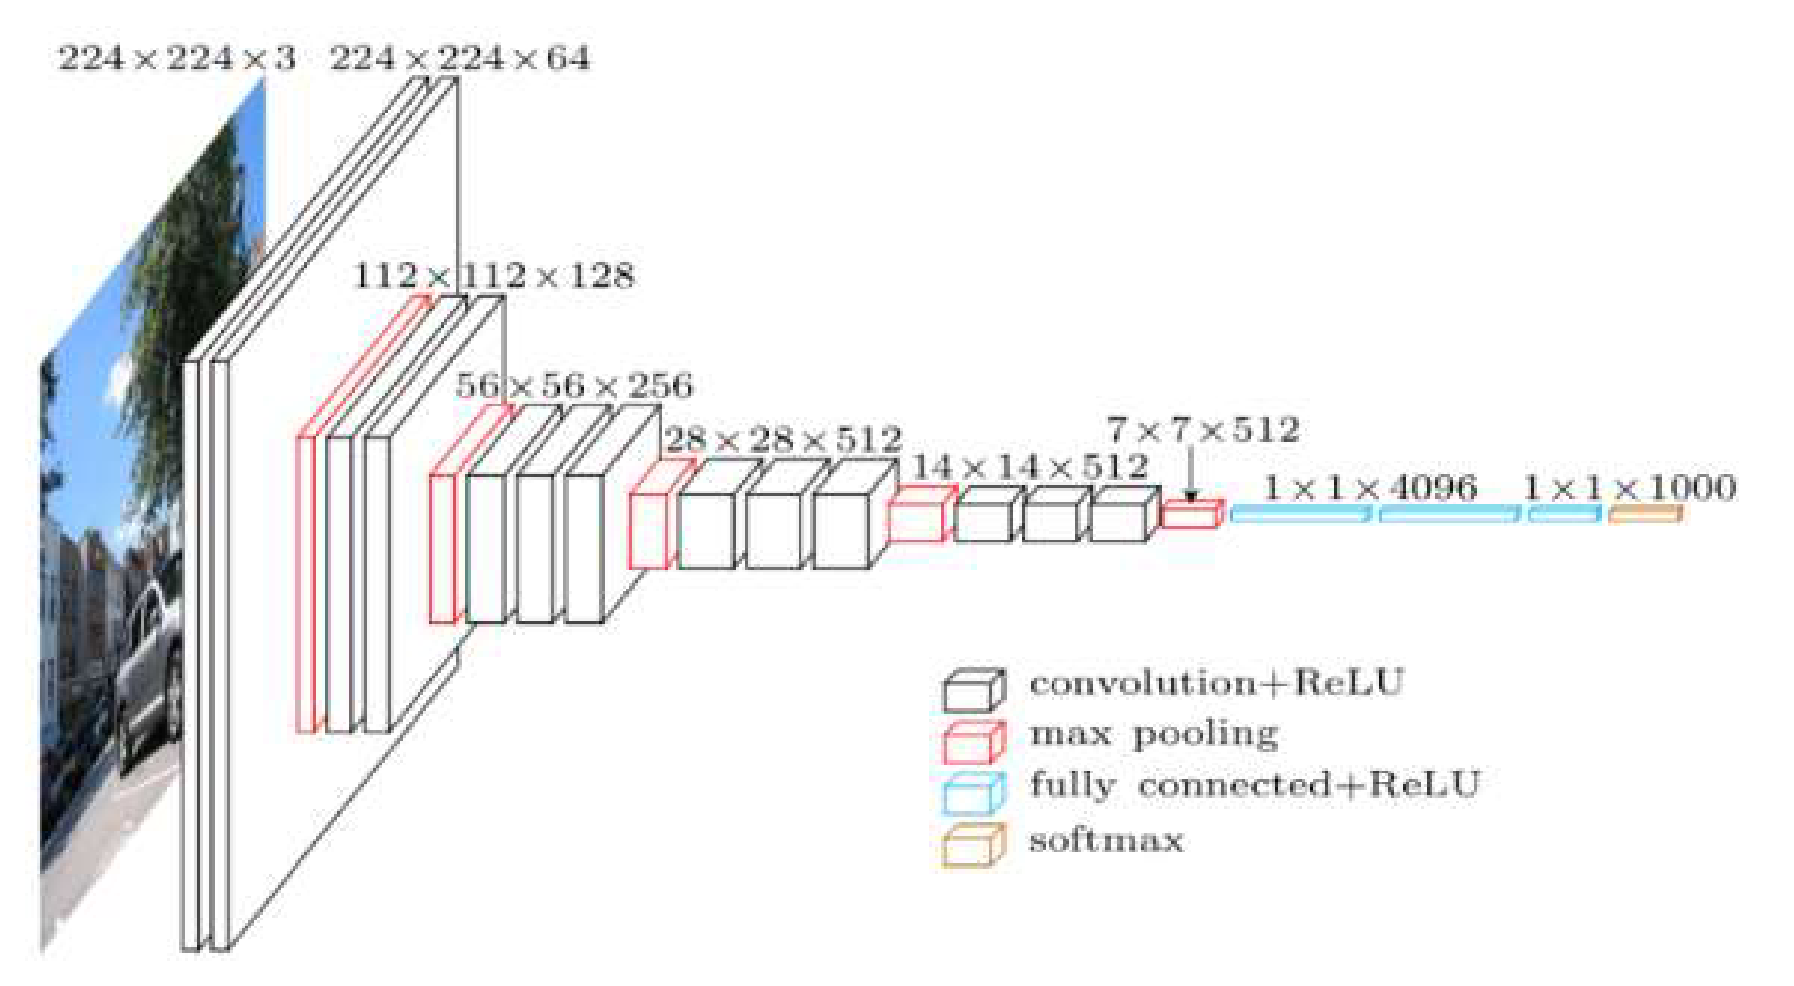
\includegraphics[width=0.8\textwidth]{images/VGG19-architecture.png}
  \caption{The structure of VGG19\cite{Simonyan15}}
  \label{fig:vgg19-structure}
\end{figure}

% TODO: add more of the models that I'm comparing and graph of the size of the models

\section{EfficientNet}

EfficientNet, developed by Google and published in the paper "EfficientNet: Rethinking Model Scaling for Convolutional Neural Networks". It was a huge leap in performance for efficient image classification models. Their primary achivement, stated in the abstract, is having 84.3\% top-1 accuracy on ImageNet, while being 8.4x smaller and 6.1x faster than the best existing convolutional neural network models.\cite{tan2020efficientnet}

\begin{figure}[ht!]
  \centering
  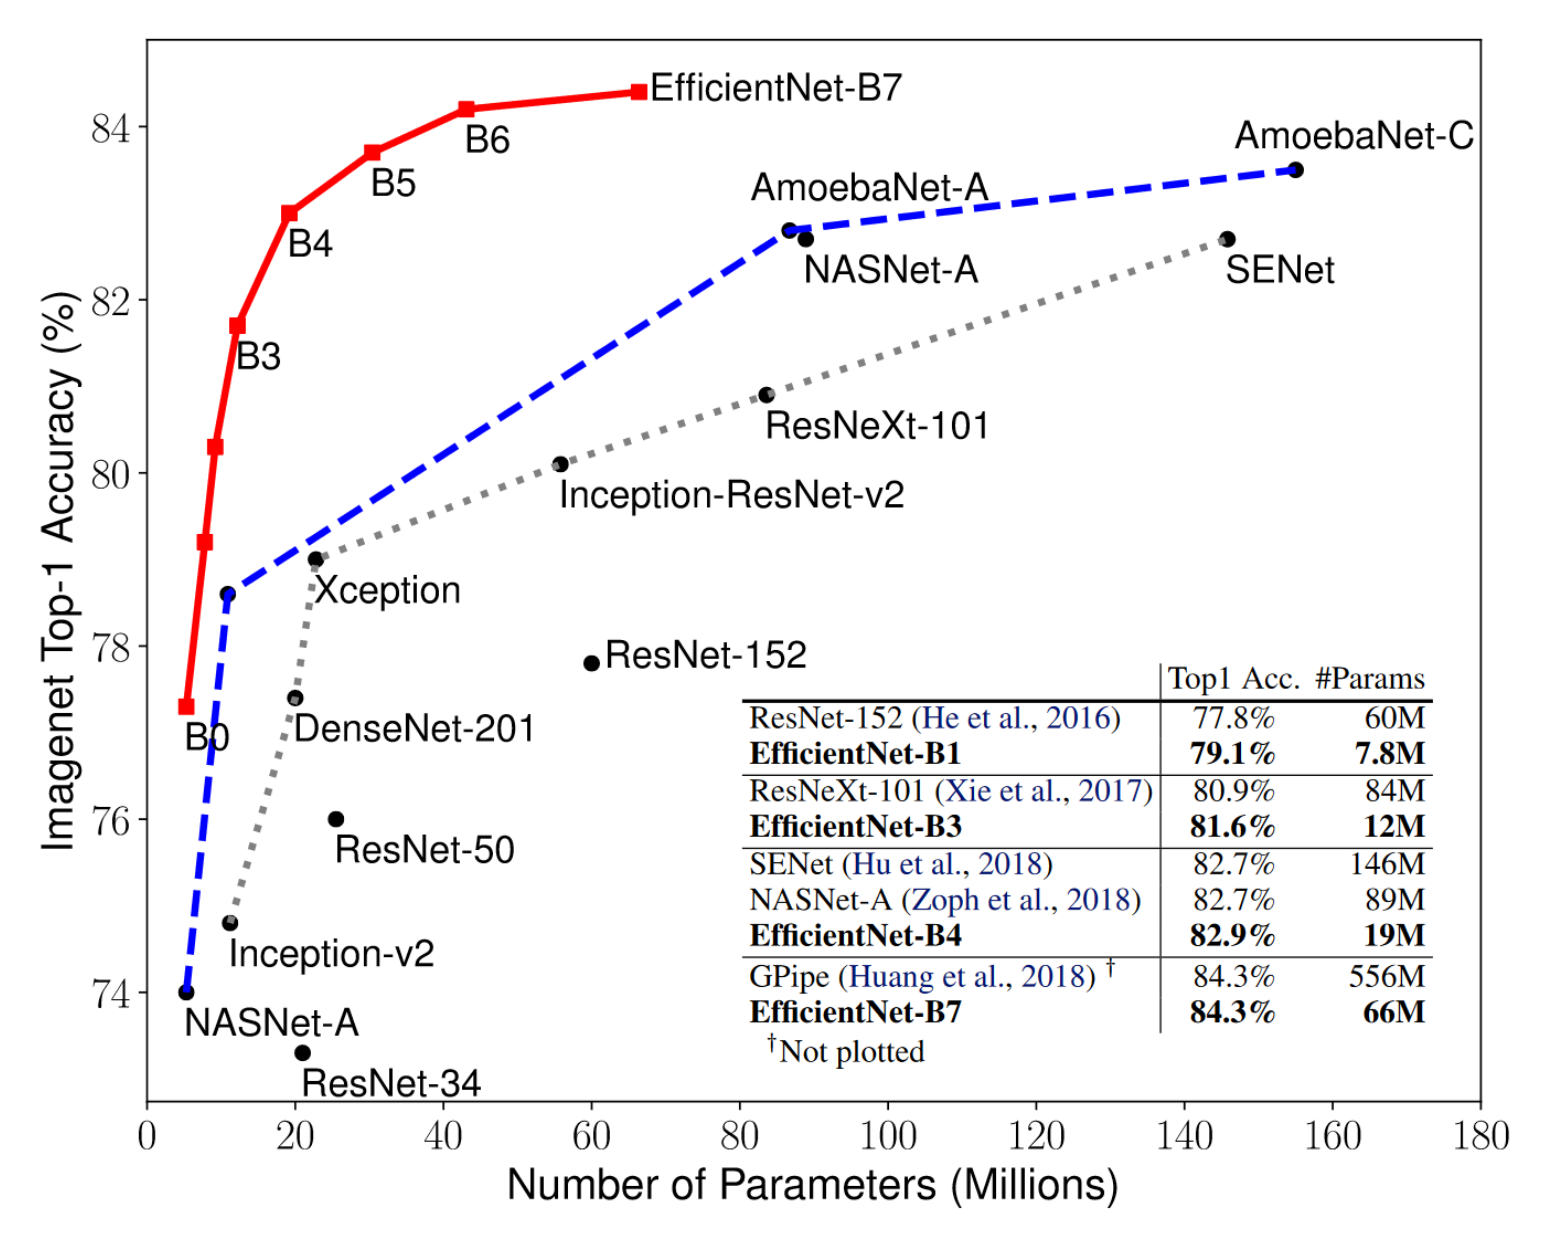
\includegraphics[width=0.8\textwidth]{images/EfficientNetComparison.PNG}
  \caption{The improvements made in the EfficientNet paper\cite{tan2020efficientnet}}
  \label{fig:efficientnet-comparison}
\end{figure}

As \ref{fig:efficientnet-comparison} shows, EfficientNet is a huge improvement over the previous models, it is much smaller, faster and more accurate than the previous models using the same techniques.

The proposal of a "compound scaling" method, which is a method of scaling the model by changing the depth, width and resolution of the model at a constant ratio, is what makes EfficientNet so much more efficient than the previous models. This is partly due to other models scaling the depth or width of the model to try and get a better accuracy, however scaling the depth of a model does normally increase it's performance, the gains are comparatively very small, as a model could double in layers, but only get a 1\% increase in accuracy. As researched in the paper "Wide Residual Networks" \cite{BMVC2016_87}, it highlights the problems with just increasing the depth of a model.

Another proposal made in the EfficientNet paper is to increase the input image resolution, as this would provide the model with more data to learn from and classify with. Unfortunately, I cannot use this method as the images that I am using are already at the maximum resolution that they can be, and increasing the resolution would not provide any additional information to the model.

\begin{figure}[ht!]
  \centering
  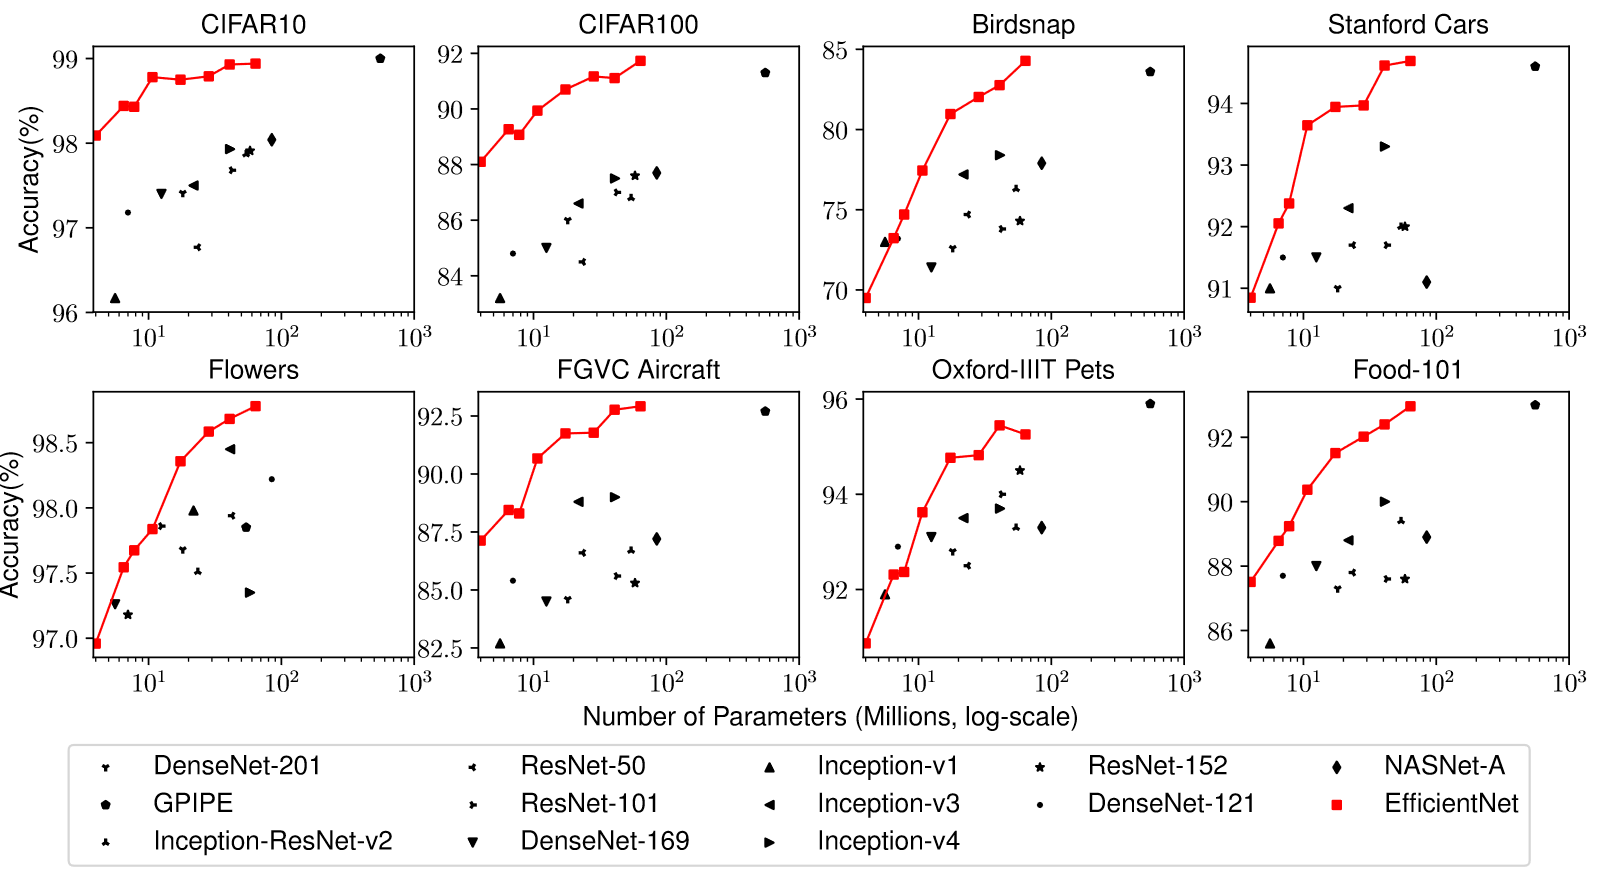
\includegraphics[width=0.8\textwidth]{images/EfficientNetPerformanceDatasets.PNG}
  \caption{The Performance of EfficientNet With Multiple Datasets\cite{tan2020efficientnet}}
  \label{fig:efficientnet-performance-with-multiple-datasets}
\end{figure}

In the figure\ref{fig:efficientnet-performance-with-multiple-datasets} it's clear to see how much better EfficientNet is than the previous models, it's much smaller, faster and more accurate than the previous models, across multiple datasets.


\begin{figure}
  \centering
  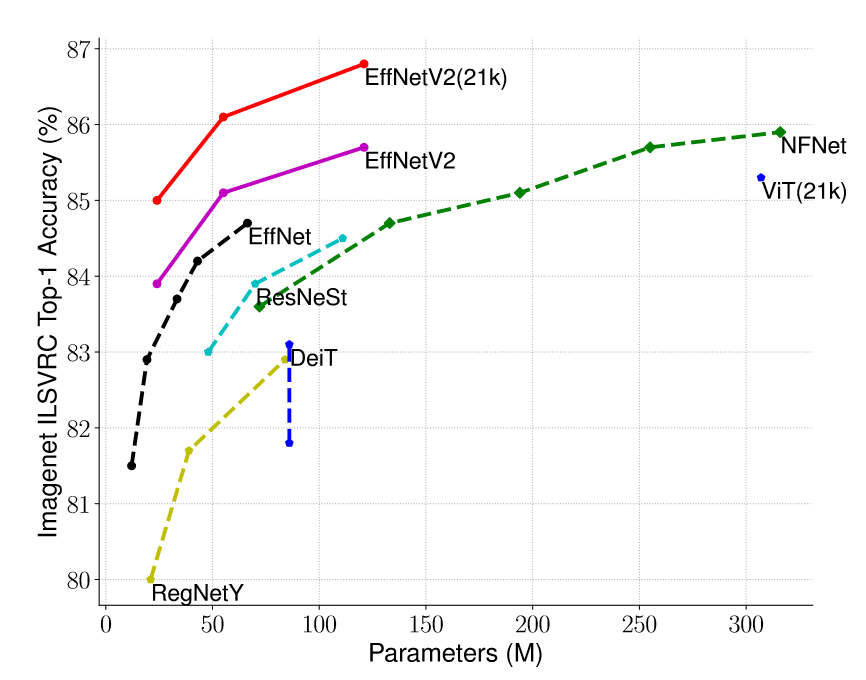
\includegraphics[width=0.8\textwidth]{images/EfficientNetv2-Performance-Graph.png}
  \caption{EfficientNetV2 \cite{DBLP:journals/corr/abs-2104-00298}}
  \label{fig:efficientnetv2-performance-graph}
\end{figure}

EfficinetNetv2: Smaller Models and Faster Training\cite{DBLP:journals/corr/abs-2104-00298} is a paper published in 2021, which is an improvement on the EfficientNet model. The top performing model in the improved group has more parameters than the original highest performing EfficientNet model, however it's top-1 accuracy goes from 84.7\% with EfficientNetB7, to 87.3\% with EfficientNetv2-XL (21k). This improvement however comes at the cost of many more parameters, from 66 million with EfficientNetB7, to 208 million with EfficientNetv2-XL (21k). The real improvement comes with the smaller models such as EfficientNetv2-S (21k) which has 22 million parameters, and a top-1 accuracy of 84.9\%, as this model has fewer parameters than the previous best EfficientNet model. \ref{fig:efficientnetv2-performance-graph} shows the performance of the EfficientNetv2 models, and how they compare to the EfficientNet models.

\section{Xception}

Xception: Deep Learning with Depthwise Separable Convolutions\cite{DBLP:journals/corr/Chollet16a} was a paper published in 2016 from Google, which introduced the concept of depthwise separable convolutions, which is a type of convolutional layer that is used in the Xception model.

\begin{figure}[ht!]
  \centering
  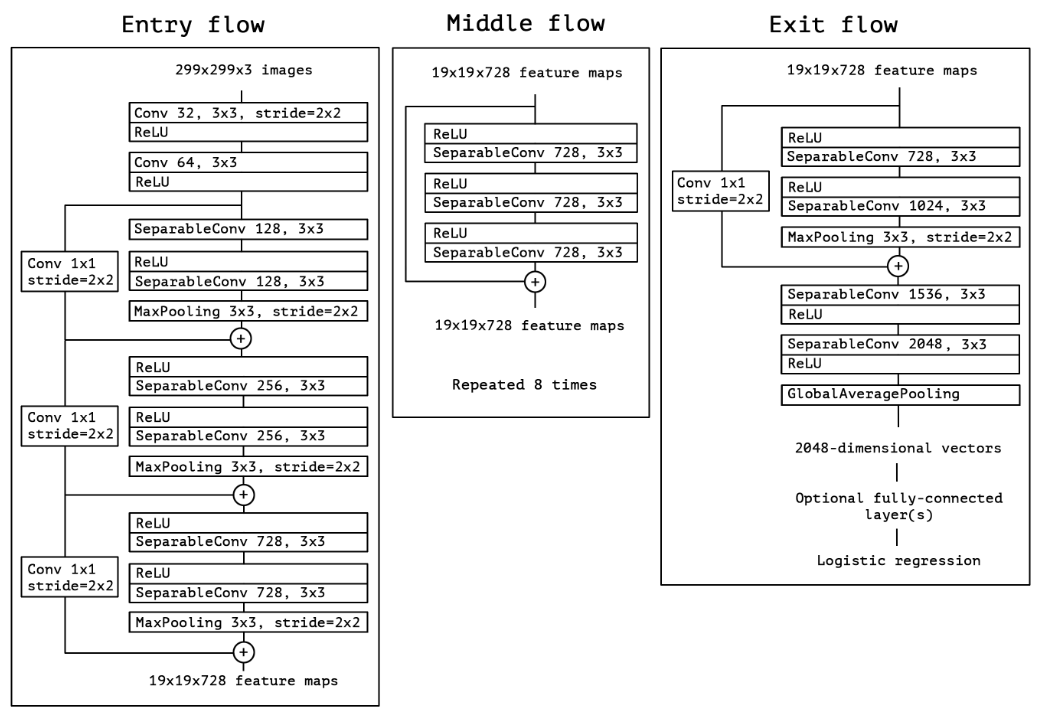
\includegraphics[width=0.8\textwidth]{images/Xception-structure.png}
  \caption{The structure of Xception\cite{DBLP:journals/corr/Chollet16a}}
  \label{fig:xception-structure}
\end{figure}

The Xception architecture is based on a novel type of convolutional operation called depthwise separable convolutions, which allow for significantly more efficient and accurate learning of features in CNNs. Regular CNNs use standard convolutional layers, which apply the same set of filters to all channels of an input volume. Depthwise separable convolutions, on the other hand, perform two separate operations: first, they apply a single filter to each input channel (depthwise convolution), and then they combine the output channels using a pointwise convolution (1x1 convolution).

This two-step process dramatically reduces the number of parameters and computations required for each layer of the network, resulting in a much more efficient architecture that can be trained on smaller datasets and run on devices with limited computational power. In addition, the Xception architecture achieved state-of-the-art results on several benchmark datasets, demonstrating the effectiveness of depthwise separable convolutions for deep learning.

\chapter{Transfer Learning}

\section{Why use Transfer Learning}
Transfer learning can enable a model to be trained much more efficiently than if it was trained from scratch, as most of the work is done by the pre-trained model.
Aside from the extra time it takes to train a model from scratch, it often requires more training data, which is not always available and can be expensive to obtain.
Transfer learning can often get better results than training a model from scratch, as the pre-trained model has already learned about different features from a large dataset,
and the transfer learning model can then use these features to learn about the new dataset.

\section{Drawbacks of Transfer Learning}
The main drawback of transfer learning is that it is not always possible to use it,
as the pre-trained model may not be able to extract the features from the new dataset.
With image classification, the pre-trained model can typically extract features from any image, but it may not be able to extract the features that are needed for the new dataset.
Transfer learning can also be less efficient than training a model from scratch,
as the pre-trained model will have all the weights from the original dataset, which may not be needed for the new dataset.
This can cause the model to be less efficient, as it will have to train on weights that are not
needed but will still affect the performance of the model.

\pagebreak
\section{The code behind the transfer learning}
The code for the transfer learning is shown below.

\begin{lstlisting}[language=Python]
  # This imports the model from the keras library
  MobileNetV3Small = keras.applications.MobileNetV3Small(
    input_shape=(224, 224, 3),
    include_top=False, 
    weights='imagenet')

  # Create the model
  model = keras.Sequential()

  # Freezing all but 10 layers of the pre-trained model
  for layer in MobileNetV3Small.layers[:-10]:
    layer.trainable = False

  # Adding the pre-trained model to the model, along with 
  # a dropout layer and a fully connected layer
  model.add(MobileNetV3Small)
  model.add(keras.layers.Flatten())
  model.add(keras.layers.Dense(512, activation='relu'))
  model.add(keras.layers.Dropout(0.6))
  model.add(keras.layers.Dense(512, activation='relu'))
  model.add(keras.layers.Dropout(0.6))
  model.add(keras.layers.Dense(4, activation='softmax'))
\end{lstlisting}

The code above shows how to create a model using transfer learning,
creating the model structure consists of adding the pre-trained model to the model,
and then adding a few layers on top of it. The Flatten layer is used to flatten the output of the pre-trained model
as that is the input for the fully connected layers. The fully connected layers are used to classify the images.

The dropout layers are used to prevent overfitting, and the dense layers are used to classify the images.
The dense layers are potentially the most important part of the model, as they are the ones that are actually learning about the dataset.
They get trained on the features extracted by the pre-trained model, and the weights of the dense layers are what is used to classify the images.

The final layer of the model is a Softmax layer, which is used to classify the images.
It is used to classify the images into one of the classes in the dataset, in this example,
the 4 levels of Alzheimer's disease that are in the Alzheimer's MRI Dataset.

\pagebreak
\section{How to implement Transfer Learning}

\subsection{Extracting features}
Feature extraction is the process of extracting features from the images in the dataset, these features
in the images could be anything, such as the colour, shape, or the texture of the image. All of these features
are used to classify the images, and having these features already extracted can make the training process much faster.
Most of the pre-trained model is usually frozen so that it does not change during the initial stages training, and only the new model is trained,
and on top of the extracted features from the base model.

\subsection{Fine-tuning}
This is the process of training the new model on the dataset, but with a lower learning rate than the initial training and the model is usually unfrozen,
so that the pre-trained model can be trained as well, which helps to improve the overall performance of the model.
This was where I managed to get the best results for my models.

\section{How to fine-tune a model}
Fine-tuning a model is a very simple process, and can be done in just a few lines of code.
The first step is to unfreeze the pre-trained model, which can be done by setting the trainable attribute of the layers to True.
The next step is to set the learning rate to a lower value, which can be done by setting the learning rate attribute of the optimizer.
The final step is to recompile the model, which can be done by calling the compile method of the model.
Here is an example of how I fine-tuned a model using Keras:

\begin{lstlisting}[language=Python]
  base_model.trainable = True
  optimizer.learning_rate = 0.0001
  model.compile(optimizer=optimizer, loss=loss, metrics=metrics)
\end{lstlisting}

\begin{verbatim}
  base_model.trainable = True
  optimizer.learning_rate = 0.0001
  model.compile(optimizer=optimizer, loss=loss, metrics=metrics)
\end{verbatim}

%\section{The different structures of the models}
%There are so many different ways to structure a model, and they can 

\section{My training setup}
For this project, I have set up my gaming laptop as a server, with Manjaro\cite{Manjaro} as the operating system.
I've chosen my laptop to do the training on due to it's powerful GPU, which is a NVIDIA GeForce GTX1070\cite{GTX1070}.
This can be used with Nvidia CUDA\cite{CUDA} to speed up the training process, which is what I have done.
Training the models on my laptop has been very useful, as it has allowed me to train the models much easier
as I can leave it to train overnight without having to constantly check on it.

I have recently upgraded the GPU in my computer to an RTX 3080\cite{RTX3080}, which is a much more powerful GPU than the GTX1070, as it has more CUDA cores, a higher core clock, 2gb more of VRAM, and a much higher memory bandwidth. Alongside this, it has "RT Cores",
these are designed to be used for ray tracing, which is a technique used to render realistic images, however they also can accelerate the training process.

\chapter{Data Importing and Preprocessing}

\section{Formatting and converting the data}
Clinica\cite{SAMPERGONZALEZ2018504} is a python library that can be used to convert the MRI scans in the different formats into the BIDS format\cite{Gorgolewski2016}.
This significantly speeds up development as the standardised BIDS format lets me use the same code for the different datasets, as well as allowing me to use pre existing tools to import the data and preprocess it, ready for training.

MRI data can be complicated and before the BIDS standardisation, it was significantly more difficult for researchers to share data with each other. It contains information such as the manufacturer of the scanner, the model of the scanner, the software associated with the scanner and version, then other parameters about the setup of the scanner, such as the field strength and the number of channels.\cite{BIDS_metadata}

Whilst I have not used the BIDS standard for all the datasets in this project, I feel that it is very useful and I will be using it for all the future datasets that I use.

\section{Dataset Augmentation}

When training a deep learning model, it is important to have a large dataset, as this will allow the model to learn from a wide variety of data.
Unfortunately I do not have as many MRI scans as I would like, so I have used data augmentation to increase the size of the dataset.
Using the ImageDataGenerator class from Keras\cite{Keras}, I have been able to generate new the new images.
This helps training the model as it allows the model to learn from a wider variety of data, and it also helps to prevent overfitting.
It is not optimal to be required to use data augmentation, however it's significantly better than not having enough data to train the model.
If these models were to be used in a real world scenario, augmentation helps to make the model more resilient to the quality of the scans.

\section{Batch sizes}
The batch size is the number of images that are passed to the model at a time.
A larger batch size will cause the model to learn quicker, however it will also use more memory whereas
having a smaller batch size will cause the model to learn slower, however it will use less memory.
When I started off, I did not understand the concept of batch sizes, and I was using a batch size of 1000, this lead to my training times
being very long and I had to wait days for a model to train.
I have found that a batch size of 32 works well for the models that I have trained and my GTX1070 8 GB GPU\cite{GTX1070} doesn't often run out of memory.

\section{Feature Normalisation}

Normalisation is the process of scaling the data so that it is typically between 0 and 1.
In the case of age, this would be the highest age in the dataset, divided by the age of the patient.
This is done to make the training process more efficient, as it helps with convergence, as it can avoid the model from getting stuck in a local minimum. This can help reduce the impact of outliers by scaling the input to a smaller range.
Although it is not required, it is generally recommended to always normalize the data.

\section{Keras Data Generators}

When passing the batched images and the other data to the model, I had to create my own superclass for the Keras Sequence class. This allowed me to pass the age, gender, MMSE score, and the image to the model, instead of just the image. I needed to create this as I did not have enough ram to load all of the images into memory, so using batches was required. This still allowed me to use the ImageDataGenerator class to augment the images.

\chapter{Evaluating the performance}

\section{The different metrics}
% Accuracy
Accuracy is typically the metric used to compare models and is defined as the number of correct predictions divided by the total number of predictions.
It is a very simple metric to understand, and is therefore often used to compare the performance of different models.
There is accuracy for both the training and validation sets, and the accuracy of the validation set is used to determine how well the model generalises to new data,
and a validation accuracy that is much lower than the training accuracy is a sign that the model is overfitting.
However, it is not always the best metric to use, as it can be misleading in some cases.

% Loss
Loss is a very common and useful method to evaluate the performance of a model, it is calculated by taking the difference between the predicted value and the actual value.
There are however many different types of loss functions, and the one that is used depends on the type of problem that is being solved.
These could be binary cross entropy, categorical cross entropy, or mean squared error. For my project I used binary cross entropy due
to it's simplicity and the fact that it is the most common loss function used for binary classification problems.

% Validation vs Training Loss and Accuracy
The validation loss and accuracy are used to determine how well the model generalises to new data, and a validation loss that is much higher than the training loss is a sign that the model is overfitting.
For the validation set, I have assigned 20\% of the data to be used.

\section{Data Augmentation}

Data augmentation is the process of artificially increasing the size of a dataset by applying random transformations or filters to the images.
This can help to improve the performance of a model, as it can help to reduce overfitting, and can also help to improve the generalisation of the model.
The transformations that are applied to the images are usually random, and can include things like rotating the image,
flipping the image, or changing the contrast/saturation of the image.

In the case of the Alzheimer's MRI Dataset, it is extremely useful to have more data to train the model on, as there are a limited number of brain scans available.
MRI scans are also very expensive, so using data augmentation can significantly reduce the cost of training the model.

In the Alzheimer's MRI Dataset, the majority of the archive consists of augmented images already however this caused me problems which I will go on to talk about.
With the flower dataset however, I did apply data augmentation to the images, as there were not enough images per class to train the model on.

\section{Problems With The Datasets and How I Fixed Them}

\subsection{The Problems}
% TODO: insert the Alzheimer's MRI Dataset images here, talk about repeated data and the problems that it causes

The Alzheimer's MRI dataset that I had chosen early on in the project was far from ideal as I found out later on.
The pre-augmentation that was applied to the dataset caused problems with the training/validation split, as the
images were already augmented, and the validation set was made up of images that were in the training set, but
with different transformations applied to them. This gave me amazing results on the validation set, but when I
tested the model on new data, it performed very poorly. Here the image shows the last 30 epochs of the training process,
and the validation accuracy is very high, higher than what other models from other research papers have achieved.

% Image of the training results
\begin{figure}[h]
  \centering
  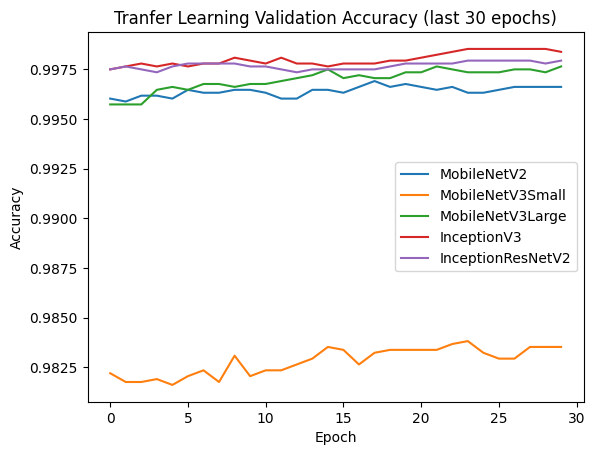
\includegraphics[width=0.7\textwidth]{images/bad-training-result.png}
  \caption{The training results from the various models (Last 30 epochs)}
  \label{fig:training_results}
\end{figure}

\pagebreak

\subsection{The solution}
The solution to this problem was to use the original images, and not the pre-augmented images.
This meant that I had to re-download the dataset, and re-split the dataset into training and validation sets,
and then apply data augmentation to the images. This gave me much better results, and the model was able to generalise
to new data much better. Here is the image of the training results from the various models, and the validation accuracy is much lower than before.

Here's the snippet of code that I used to augment the images:
\begin{lstlisting}[language=Python]
train_datagen = ImageDataGenerator(rescale=1./255,
    validation_split=0.2,
    featurewise_center=True,
    featurewise_std_normalization=True,
    rotation_range=360,
    width_shift_range=0.1,
    shear_range=0.1,
    zoom_range=0.1,
    height_shift_range=0.1,
    horizontal_flip=True,
    vertical_flip=True,
)
\end{lstlisting}

\pagebreak

This however did not solve all my problems, as the model was still overfitting. This ended up being a problem with the dataset, as even with the "original images" that were provided, there were still images that were repeated, and aside from the overfitting problems this caused, it also meant that my validation set had images that were in the training set, and this gave me very high validation accuracy.

This was then solved by going directly with the OASIS-1 dataset, and using the images that were provided there. I was hesitant to do this at first, as there was more pre-processing required to format the data in the way that I wanted it, but it has now allowed me to train my models without getting false results.

By using the OASIS-1 dataset directly, that presented a new set of challenges, as the images were given in a different format, as I had a CSV file with the labels and the image IDs which identified the images. This lead me to learn how to use the Pandas\cite{Pandas} library in Python, which allowed me to read the CSV file and extract the image IDs and the labels from it. Then I had to create my own custom data generator, which allowed me to load the images from the dataset, and apply the transformations to them. This was a very useful learning experience, as I was able to learn important skills relating to data preprocessing. The data generator, which I had talked about earlier, helps batch and augment the data that is being fed into the model during training.

\section{Evaluating the given metrics}
The metrics of accuracy and loss generally tell us how well the model is performing,
but they do not tell us how well the model is performing for each class.
They do also not tell us how well the model would work in a real world scenario,
as they are only calculated on the training and validation sets, of which we have a limited amount of data.

The validation dataset is also from the same distribution as the training dataset,
so it is not a good representation of how well the model would work in a real world scenario
as the scans could be of a different quality.

I have used the augmented dataset for the training and validation sets as this
should give a better representation of how well the model would work in a real world scenario.


% TODO: TALK ABOUT METRICS


\pagebreak

\chapter{Software Engineering}

\section{The code}
The way I have structured the code is by having a main.py file that contains the code to train the model, and a Main.ipynb file that contains the code to test setting up the model.

\subsection{My Development Python Environment}
% TODO: edit this section and make it more concise and descriptive of the final project
I have used the following tools to develop this project:
\begin{itemize}
  \item Python 3.8.5\cite{Python} - To run the code
  \item Jupyter Notebook\cite{Jupyter} - To help me develop the code and generate the graphs
  \item Visual Studio Code\cite{VsCode} - As my IDE to develop in, I have used the SSH feature of VsCode to SSH into my Linux server and modify the code there quickly
  \item GitLab\cite{RHULGitLab} - To store the code and to track the changes
  \item tmux\cite{tmux} - To run the code in the background
  \item CUDA\cite{CUDA} - To train the models on the GPU
\end{itemize}

\section{My Web Development Environment}

For the web development, I have decided to use Typescript + React. This is because I have experience with these from my previous projects, and I wanted to use a framework that I was familiar with. I specifically used a template\cite{TypescriptProjectTemplate} that I created in a previous project, and I have used this template for this project too.

I have used the following libraries to develop the front end in this project:
\begin{itemize}
  \item React\cite{React} - To create the web application
  \item Typescript\cite{Typescript} - To add types to the code
  \item TailwindCSS\cite{tailwindcss} - To style the web application quickly
  \item Vite\cite{Vite} - To bundle the code and to run the development server quickly
  \item MaterialUI\cite{MaterialUI} - To use the Material Design components
  \item TensorflowJS\cite{smilkov2019tensorflowjs} - To run the model in the browser
\end{itemize}

\section{Using Git}
I have used Git to manage the code, and have used the RHUL GitLab server to host the code.
This was not the first time I have used Git, however it was the first time I have used it with GitLab.
I used separate branches for the different stages of the project, and then merged them into the master branch when they were complete.
The branches were made to create the different planning papers, and then to set up the development environment.
I also used branches to create the different models, and then to test them too.

All of my commits were in the format of Commitlint\cite{CommitLint} to make it easier to read the commit messages, make them more consistent,
and to make it easier to go through the history and find a specific change or commit to cherry-pick or revert.
I have tried to make my commits small and concise, and to try to make sure that each commit is a complete change.
This makes it easier to revert a change if it breaks something, and it makes it easier to cherry pick a change if it is needed in another branch. I have cherrypicked a few commits throughout the project, however when I need to use it, it comes in very handy.

I have also used GitKraken\cite{GitKraken} to help me manage the code, and to make it easier to see the changes that I have made, handle the Git tree and to make it easier to merge the branches.

\section{Testing with Jupyter Notebook}
I have used Jupyter Notebook to test the code, and to generate the graphs.
This was the most useful tool for me as it allowed me to test the code quickly and easily,
I had many issues with setting up the code as this was the first time I have trained any model.

\subsection{Using Test Driven Development}
I used PyTest\cite{PyTest} to test the code, and to make sure that everything was working as expected.
This helped me quickly test and debug my code, I would write a test to define how I wanted my code to work, and then write the code to make the test pass.
This sped up development as I could quickly test the code and make sure that it was working as expected.

The other tests I wrote were making the graphs that I generated, as I was testing the code by generating the graphs using Jupyter Notebook\cite{Jupyter} and matplotlib\cite{Matplotlib},
and then checking that the graphs were looking correct. This was really the only way I could test the training code, as the models take 10+ hours to train,
and I didn't have the time to train the models multiple times to see if unit tests that I had written were correct.

In the future I would like to use unit tests as I could set up an automated pipeline to train the models and then run the unit tests,
and then if the unit tests fail, then the pipeline would fail, and I would be notified. This would allow me to test the code more easily,
and to make sure that the code is working correctly. I would also be able to test the code on a smaller dataset, which would allow me to train the models quicker,
and to test the code quicker.

Aside from testing the models, I could set up unit tests for an API that I could create for anyone to upload their brain scans to and get a prediction of whether they have Alzheimer's or not.
This would give me an opportunity to write unit tests for the API, and to test the code that I would write for the API.
% TODO: Talk about the api and the tests

\subsection{Different learning rates}

When training a model, the learning rate is the rate at which the model learns from the data.
A low learning rate will cause the model to learn slower, and a high learning rate will cause the model to learn quicker
but it can also cause the model to get stuck in a local minimum. A combination of a high learning rate whilst the base model is frozen, and a low learning rate whilst the base model is unfrozen is a good way to train a model as it allows the model to learn quickly at the start, and then fine-tune the model at a slower rate.

A local minimum is when the model can't decrease its loss any further by adjusting its parameters.
It is stuck at a 'valley' in the loss landscape with the parameters that it currently has.
A global minimum is the same concept, but it is the absolute lowest the model can take its loss.
It is the lowest point in the entire loss landscape no matter what parameters the model has.

% Also talk about the different learning rates and how they affect the performance of the models

\section{Frontend Typescript and React}

For the frontend, I have chosen not to use TDD as it would be difficult to test the code, as it's mostly just displaying the results from the the models that I have trained. I did however setup the project using my template\cite{TypescriptProjectTemplate} that I created prior to this project, which has a basic setup for a React Typescript project, which used EsLint\cite{EsLint} to format the code and to make sure that the code is consistent, and to make sure that there are no syntax errors.

Defining the types for the data that I am using was very useful, as it allowed me to see potantial errors in the code before I even ran it, and it allowed me to see what data I was working with, and what data I was expecting to get back from the functions that I was using. This saved me a lot of time as I didn't have to go through the code and try to figure out what was going wrong.

The component based architecture of React made it easy to create the frontend and the routing for the different pages. It allows me to have a format and standard layout for the different pages, and it makes it easy to add new pages and to add new components to the pages, alongside importing different libraries and packages which can speed up development.

I have used React\cite{React} as it is a popular framework for creating web applications, and I've got experience with it. It specifically uses React Typescript, which is a combination of React and Typescript. Typescript is a superset of Javascript, and it adds types to Javascript.
This allows for better code completion, and it makes it easier to debug the code, as it will tell you if you've made a mistake sooner, whereas javascript would give you an error at runtime, if you end up with a type error. Typescript helps counter many of the issues with JS however it's not perfect and there are still issues where there can be scope for errors.

I do have the option of using tensorflow-JS, which can process all of the data locally, this has benefits and drawbacks, the main benefit is that the user doesn't have to upload their data to a server, which can make the handling more secure as everything is processed locally, so there would be far less red tape with data protection laws. The main drawback is that the model would have to be downloaded to the user's device, which could be a problem if the model is large, and it would also mean that the user would have to wait for the model to be downloaded before they could use the application, then they would have to wait for the model to make a prediction after this.

I've decided to use Python for the API backend, as it's the main server side language I have used so far. I can use Flask to host the api and return the results when they have been processed by the model.

Although I had developed the API in Python, I decided to use the TensorflowJS library to process the data, as it would be easier to use, and it would allow me to program more efficiently and host the project on a static website, which would make it easier to host and maintain.

\section{How I'm Going To Get My Results}

The way I'm going to get the bulk of my training results will be with my testing and training class that I have created. This is to help speed up the training process, as I can set the parameters that I want to use for augmentation/traning, then I can run the training and testing class, and it will put the results into seperate JSON files which I can then use to generate the graphs and tables that I need for my report. It also saves the models, so I can use them later on if I need to.

For more specific results, I would have liked to use the scikitLearn library with a GridSearch to find the best parameters for the model, however I didn't have time to do this, and it would have been very inefficient.
I ended up training a model, then using that model to train for more epochs with varying parameters, to try and narrow in on the best parameters for training the model.
This method worked well, as I could get the majority of my results automatically, leaving it running overnight, then specialising the model for more epochs with different parameters.

\chapter{Identifying and Mitigating Bias}

\section{The OASIS-1 Dataset}
The OASIS-1 dataset\cite{OASIS} that I used for this project contains 416 patients with 434 scans.

\subsection{nWBV vs Age}
Giving the age of the patient to the machine learning algorithm may allow for bias, this is because there are very few patients who are young and have Alzheimer's disease, in the dataset.
This also means it would likely be problematic to give the normalized whole brain volume to the machine learning algorithm, as this is likely to be highly correlated with age, and will therefore allow for bias.

\begin{figure}[h]
  \centering
  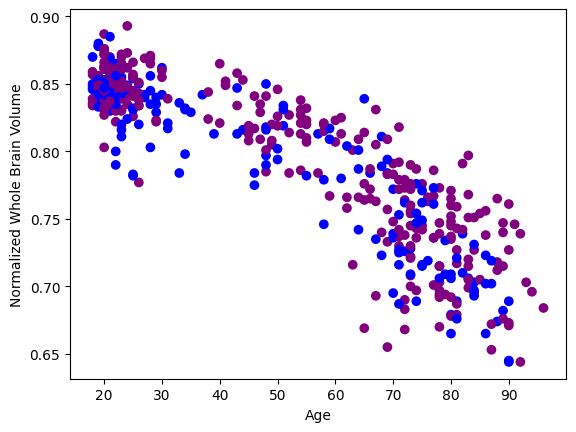
\includegraphics[width=1\textwidth]{images/nWBV-vs-Age.png}
  \caption{The nWBV of the patients in the dataset}
  \label{fig:nWBV-vs-Age}
\end{figure}

\clearpage
\subsection{eTIV vs Age}
This scatter graph is significantly more random than the one for age and whole brain volume, which means it is likely better to give to the machine learning algorithm, as it shouldn't give any strong indication of the age of the patient, and it should be useful for the machine learning algorithm.
One potential issue with this parameter is that women are more likely to have Alzheimer's disease, and this graph shows how the men and women are separated, which may allow for bias based off of the gender of the patient.
\begin{figure}[h]
  \centering
  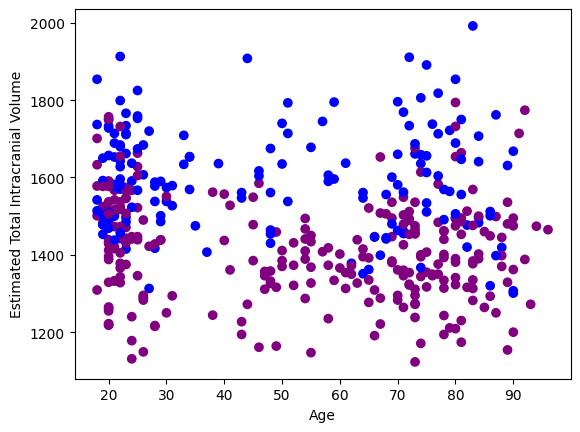
\includegraphics[width=1\textwidth]{images/eTIV-vs-Age.png}
  \caption{The eTIV of the patients in the dataset}
  \label{fig:eTIV-vs-Age}
\end{figure}

\clearpage

\section{The Skin Cancer Dataset}
The Skin cancer dataset that I was provided for this project contains images of benign and malignant skin cancer.

% Show the benign and malignant images
\begin{figure}[h]
  \centering
  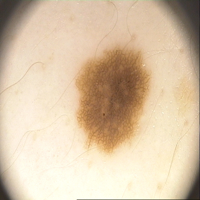
\includegraphics[width=0.2\textwidth]{images/benign-skin-cancer.png}
  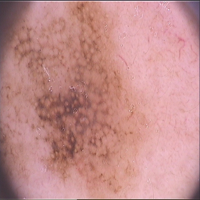
\includegraphics[width=0.2\textwidth]{images/malignant-skin-cancer.png}
  \caption{Benign and malignant skin cancer image}
  \label{fig:benign-malignant}
\end{figure}

These are some example images of what the training and test data looks like. The images are all 200x200 pixels and are in RGB format.
Unfortunately they appear to only be pictures of caucasian skin, which means that the model may not be able to predict skin cancer on people with other ethnic backgrounds.
There does however appear to be multiple types of skin cancer in the dataset, which means that the model should be able to predict a variety of skin cancers.
With this particular dataset, I don't have the ability to do much to mitigate bias, as the dataset is already biased towards caucasian skin, and my points of reference for model accuracy are with this dataset.
This dataset is also relatively small, with only 484 images all together. Although this is a small number, the results from training with this dataset are still very good, and the model is able to predict skin cancer with a high accuracy, it just have slightly more bias than it would if it was trained with a larger and more diverse dataset.

\chapter{My Initial Faulty Training Results}

This section was given from the point of view that the faulty dataset was not faulty, and that the results were genuine.

\subsection{The Comparison Of The Different Models}
Here is a graph of all the different models that I have trained properly with the old and faulty Alzheimer's dataset from kaggle.
The graph shows the accuracy of the models on the validation set along with the accuracy on the training set.
\begin{figure}[h]
  \centering
  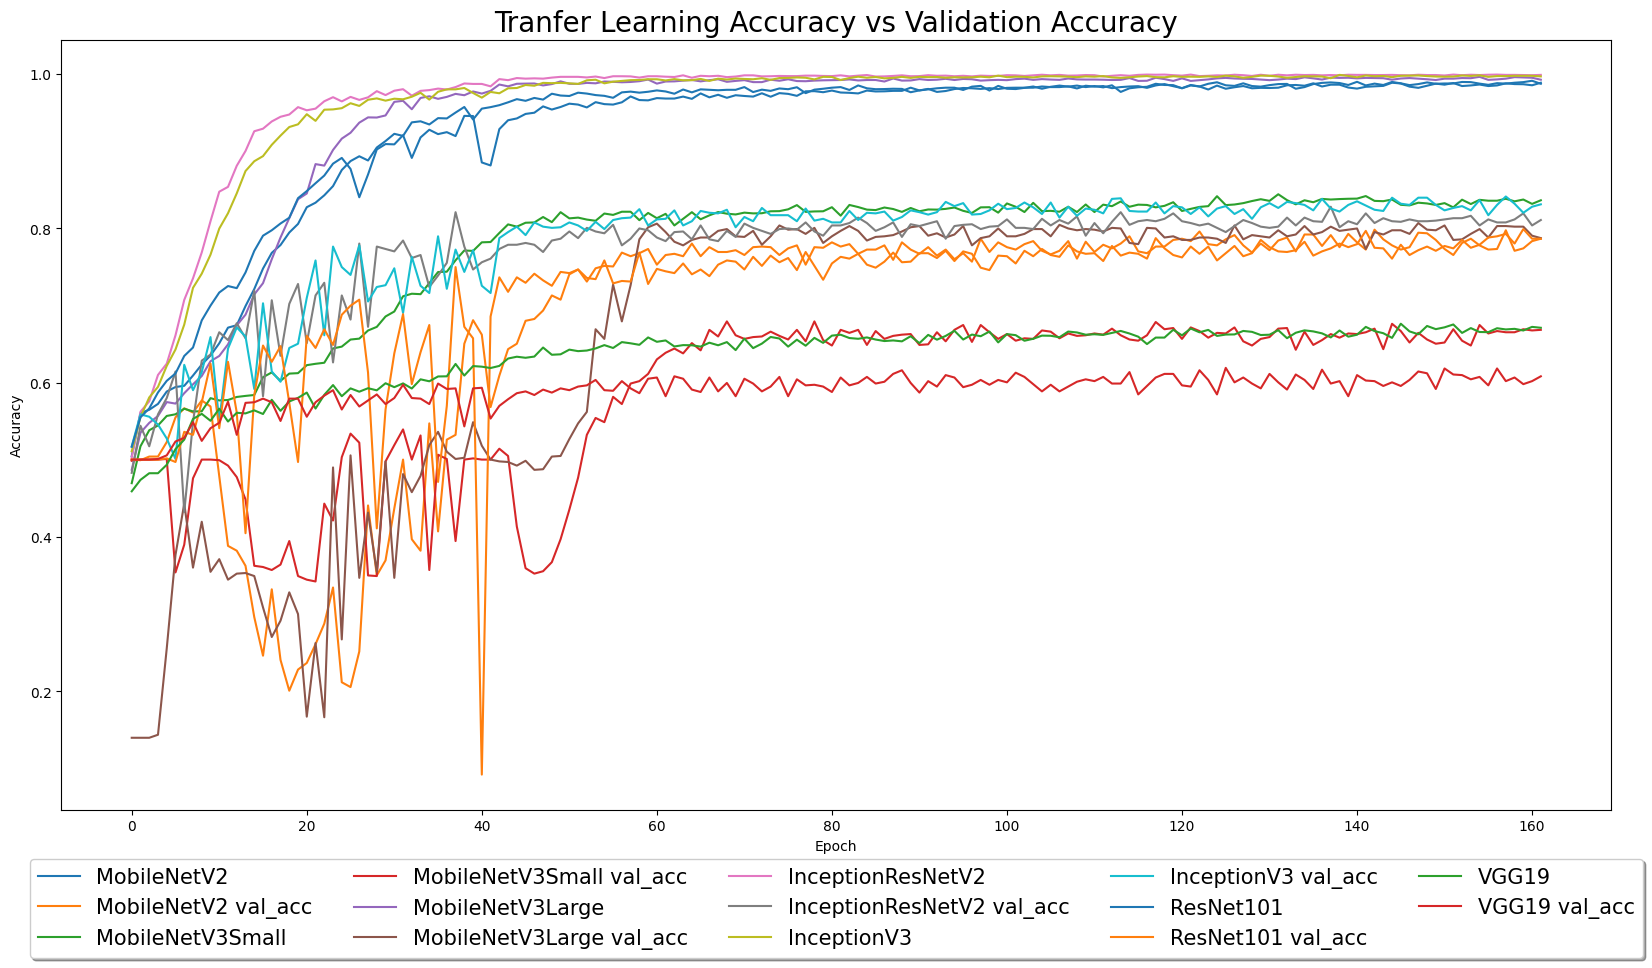
\includegraphics[width=1\textwidth]{images/good-training-acc-vs-val.png}
  \caption{The accuracy of the different models}
  \label{fig:loss}
\end{figure}
\pagebreak

\subsection{InceptionV3}
For my training results, when everything was working correctly, I was able to get the highest validation accuracy of 84\% and a loss lowest of 0.30.
% Show the graphs of the training results
\begin{figure}[ht!]
  \centering
  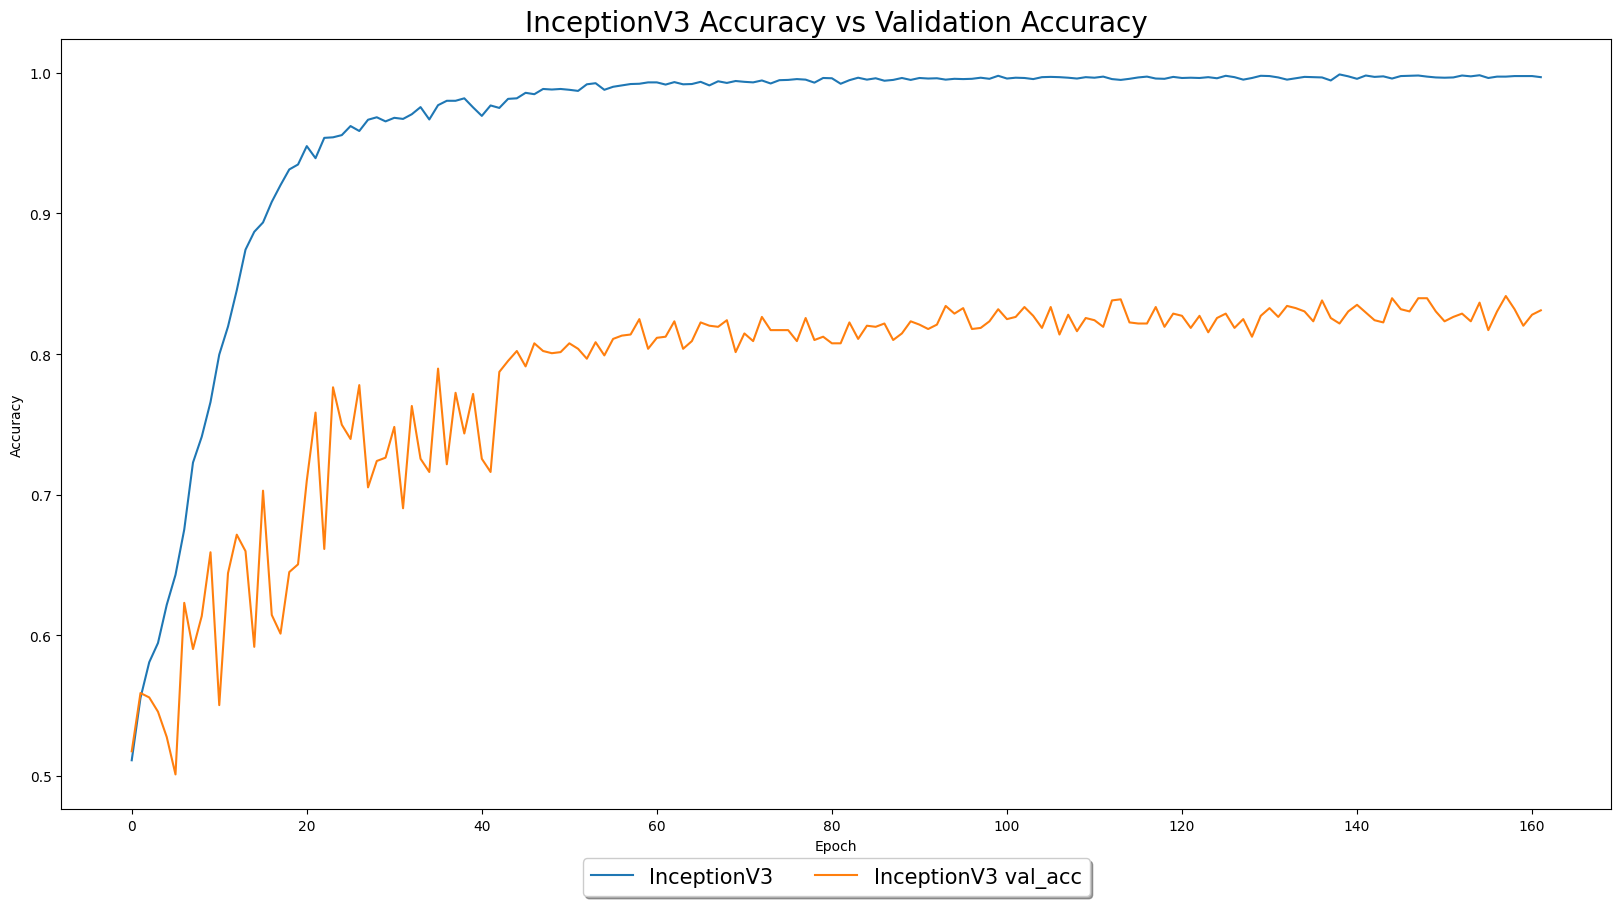
\includegraphics[width=120mm]{images/inceptionv3-accuracy-vs-val-acc.png}
  \caption{The training results using InceptionV3\cite{DBLP:journals/corr/SzegedyVISW15} as the base model}
\end{figure}

This graph clearly indicates that there was overfitting, as the validation accuracy is significantly lower than the training accuracy.
This is due to the fact that the model is learning from the training data, and it is not generalising well to the validation data.
To help mitigate overfitting, I did use data augmentation and dropout layers, however I think that the base model it's self is overfitting to the data.

I was planning on using L2 and L1 regularisation techniques work by adding a penalty to the weights of the model, which helps to reduce overfitting, however I didn't have to implement as I changed from this dataset to the OASIS-1 dataset.
Hyperparameter tuning is a process of optimising the hyperparameters of a model, such as learning rate, number of layers, etc.
This helps to improve the accuracy of the model and reduce overfitting.


\pagebreak

\subsection{MobileNetV3 Small}

MobilenetV3 Small is the smallest model in size and is consistently the least accurate model and has the highest loss.

% insert graph of loss
\begin{figure}[ht!]
  \centering
  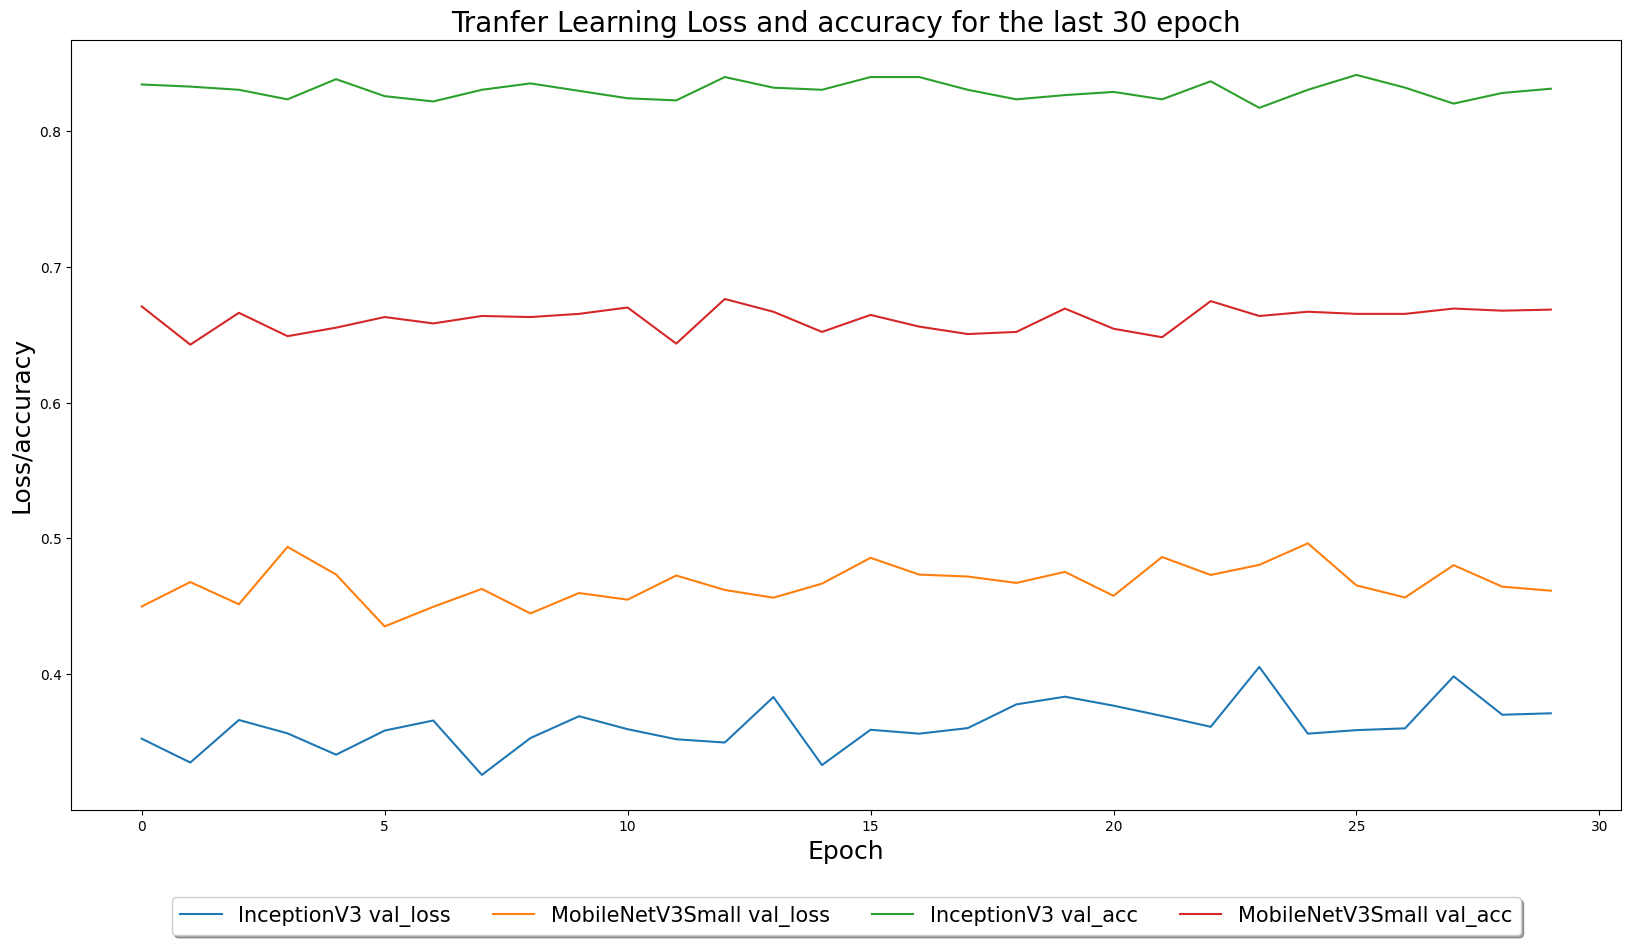
\includegraphics[width=120mm]{images/mobilenet-v3-small-vs-inception-v3.png}
  \caption{The last 30 epochs of the training results}
\end{figure}

Here's another graph that clearly shows the difference in performance between Inceptionv3 and MobilenetV3 Small.
Although InceptionV3 is slightly over 2x the size of MobilenetV3 Small, the model is likely not overfitting as much as the other models are, however I can't be sure as this was trained with the old dataset.

\pagebreak

\subsection{The model sizes}

Here's a bar chart comparing the sizes of the models in megabytes.
They are uncompressed and include the full model, after transfer learning.

\begin{figure}[ht!]
  \centering
  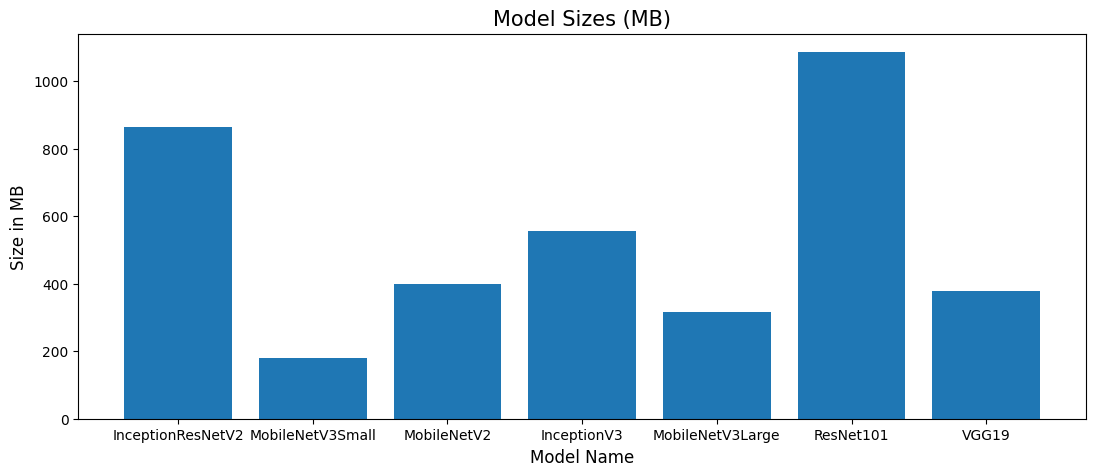
\includegraphics[width=120mm]{images/model-sizes.png}
  \caption{The different model sizes in MB}
\end{figure}

From this graph, it's clear to see how large some of the models are in comparison to each other.

\begin{figure}[ht!]
  \centering
  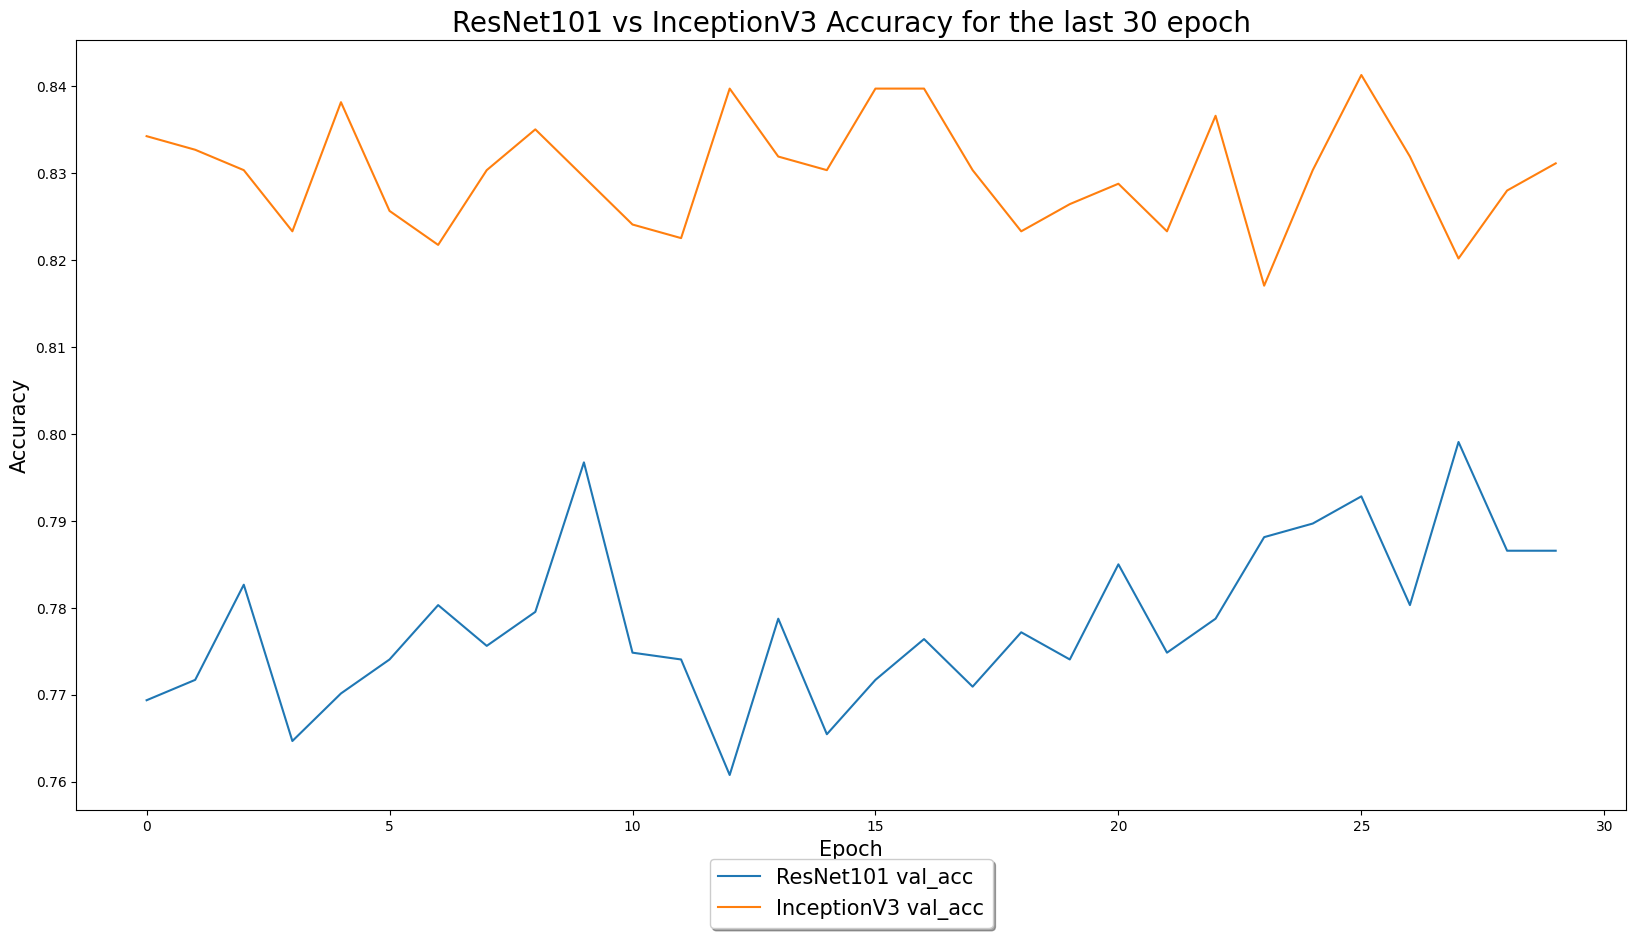
\includegraphics[width=120mm]{images/ResNet101-vs-Inceptionv3.png}
  \caption{Here's it's performance in comparison to InceptionV3}
\end{figure}

The ResNet101\cite{DBLP:journals/corr/HeZRS15} model was created by Microsoft and is a 101 layer deep neural network.
It was created to compete in the ImageNet Large Scale Visual Recognition Challenge\cite{ILSVRC} in 2015.
Inceptionv3 is a 48 layer deep neural network, and was created by Google to compete in the same challenge in 2015.

\section{Why These Results Looked Promising}
The results from the faulty dataset looked so promising as there was consistent progress in the accuracy of the models, and the loss was decreasing over time. This was because the model was learning from some of the validation data (but not all) so it's accuracy was never perfect (100\%) on the validation data, but it was high enough to give the illusion that the model was working well.

My lack of experience with machine learning meant that I didn't know what to trust when it came to the results, I just assumed that the model was working well. Thankfully I did realise the issue before I had finished my project, and I was able to fix it with the upcoming results.

\chapter{The new training results}
% TODO: train the models again with the new dataset and parameters, then show the results here

\section{The OASIS-1 Dataset}

The OASIS-1 dataset accuracy is not particularly high without any optimization, the 2D preprocessed scan images don't provide enough information for the transfer learned models to learn from and make accurate predictions.

\subsection{Training with only the MRI scans}

Training the different models with only the MRI scans as the input data was not very successful, as the models were not able to learn from the data and make accurate predictions. 

\begin{figure}[ht!]
  \centering
  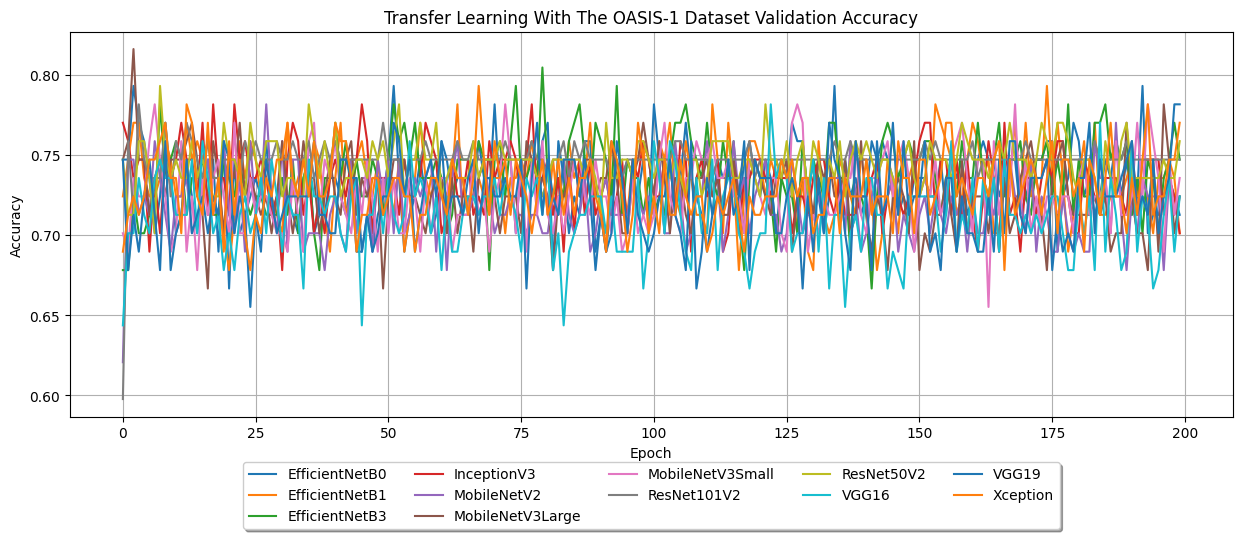
\includegraphics[width=1\textwidth]{images/OASIS-1-Transfer-Learning-Basic-Results.png}
  \caption{The results of training the models with only the MRI scans}
  \label{fig:OASIS-1-Transfer-Learning-Basic-Results-Accuracy}
\end{figure}

In \ref{fig:OASIS-1-Transfer-Learning-Basic-Results-Accuracy}, the graph shows all the validation accuracies of the models. This clearly shows there was no model that performed well, as the highest accuracy only peaked at 80\% and the majority of the time, the models were around 75\% accuracy. This would not be too bad, if the dataset were not imbalanced, however it is, as there are around 3 times more healthy patients than there are patients with Alzheimer's disease. This means it can just predict that everyone has AD and still get a 75\% accuracy. 

The validation loss in \ref{fig:OASIS-1-Transfer-Learning-Basic-Results-Validation-Loss} tells a similar story too, there really aren't any gains made past the 75th epoch, by any of the models and the loss is just stuck around 0.6 for the majority of the time. This means that the models are not learning from the data, the training loss and accuracies continue to improve however this just suggests to me that they are overfitting to the training data.
 
% Show the val loss graph
\begin{figure}[ht!]
  \centering
  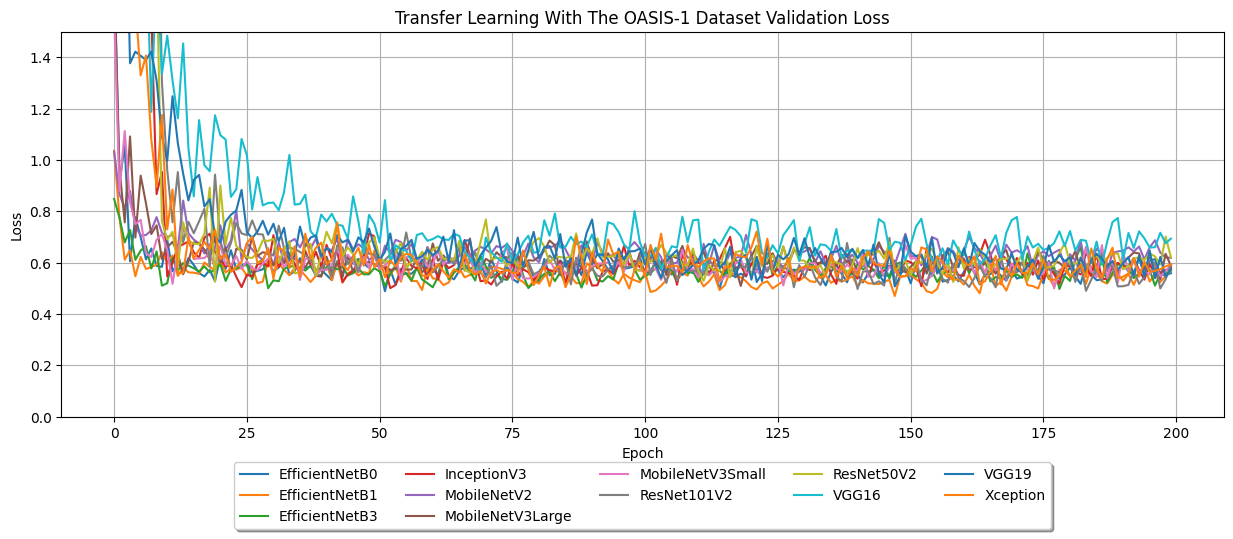
\includegraphics[width=1\textwidth]{images/OASIS-1-Transfer-Learning-Basic-Results-val-loss.png}
  \caption{The results of training the models with only the MRI scans}
  \label{fig:OASIS-1-Transfer-Learning-Basic-Results-Validation-Loss}
\end{figure}

\subsection{Training with the MRI scans and the other features}

Training models with more than just the MRI scan led to much more promising results, here is the loss graph from one of the models I had chosen to train with the MRI scans and the other features \ref{fig:VGG19-OASIS-1-loss}.

\begin{figure}[ht!]
  \centering
  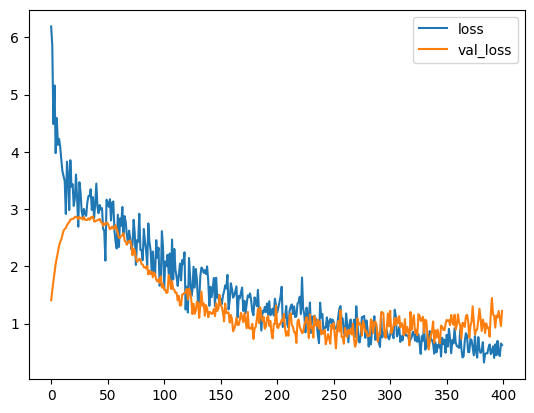
\includegraphics[width=0.5\textwidth]{images/VGG19-OASIS-1-loss.png}
  \caption{The results of training the models with the MRI scans and the other features (VGG19 model)}
  \label{fig:VGG19-OASIS-1-loss}
\end{figure}

In figure \ref{fig:VGG19-OASIS-1-800-epoch}, it is clear to see that the model is not learning any more from the data, and the model has slightly overfit to the training data. This may be because I could not augment the other inputs, such as age, as that would not make sense. Although the model is overfitting, it's validation accuracy is peaking at around 93.10\% which is far better than the 75\% accuracy of the models trained with only the MRI scans.

Although these results look better, I believe that this may just be because the dataset is imbalanced, and the model could just be predicting that someone may have Alzheimer's disease based off of their age, or other factors which corrolate with an increased risk of Alzheimer's disease, rather than it detecting the potential causes of Alzheimer's disease in the MRI scans.

\begin{figure}[ht!]
  \centering
  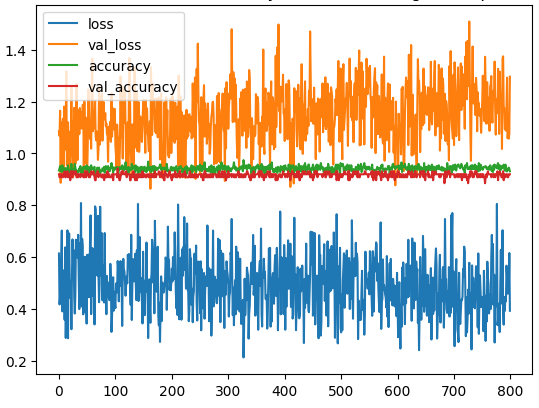
\includegraphics[width=0.5\textwidth]{images/VGG19-OASIS-1-800-epoch.png}
  \caption{The fine tuning results of training the models with the MRI scans and the other features (VGG19 model)}
  \label{fig:VGG19-OASIS-1-800-epoch}
\end{figure}

\pagebreak

\section{How this could be improved}

I believe that with a dataset such as the OASIS-3 dataset, which has more balanced classes, and more data, the models would be able to learn from the data and make more accurate predictions. This is because there are very few people with severe Alzheimer's disease, and the majority of the people in the dataset have no Alzheimer's disease.



\section{The Skin Cancer Dataset}
Training the models with the skin cancer dataset was a lot more successful than training with the other dataset. This is likely due to the fact that skin cancer is visually easier to identify than Alzheimer's disease, as the skin cancer images are much more clearly defined.

\begin{figure}[ht!]
  \centering
  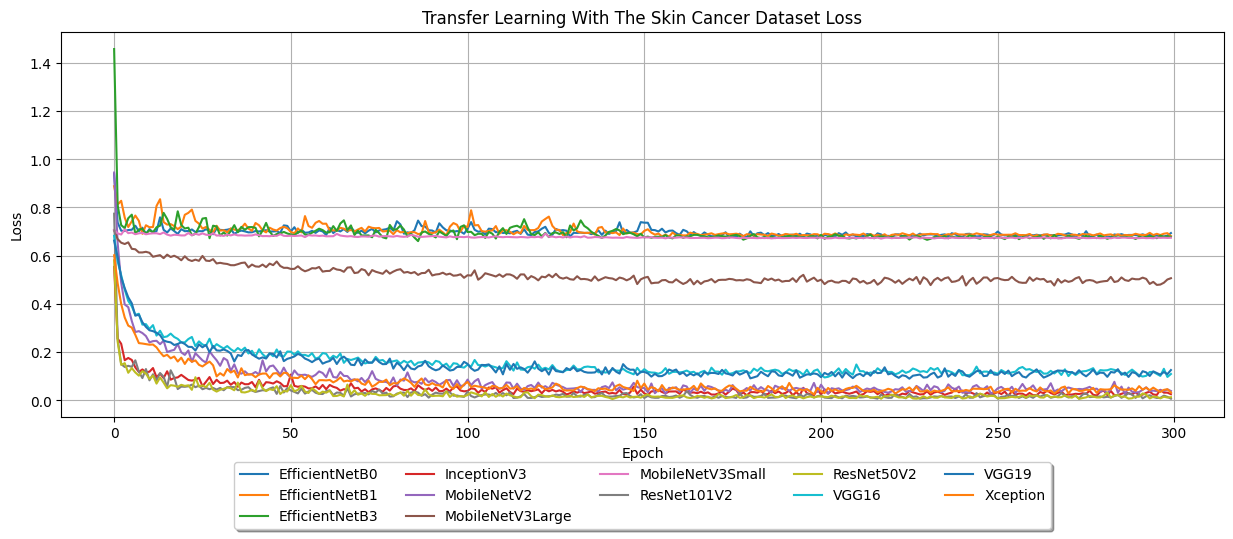
\includegraphics[width=1\textwidth]{images/skin-cancer-loss.png}
\end{figure}

As this graph shows, there are lots of models that did well, and a handful that did poorly. This is only the loss from the training data, and not the validation data, so it's only really a good indication of what models obviously performed poorly, such as the EfficientNetB3 and the MobilenetV3 models.

\pagebreak

\begin{figure}[ht!]
  \centering
  \includegraphics[width=1\textwidth]{images/skin-cancer-validation-accuracy-last-50.png}
\end{figure}

This graph shows the last 50 epochs of the training process for the skin cancer dataset, with the validation accuracy. This shows the most clear results, as the models with a high accuracy here are the ones that have learned the best from the training data.
This was graph was also created with the full augmentation performed on the validation data. This may have changed the results to make the models appear to perform worse than they actually did, however lots of the augmentation I had done was reasonable and within the scope of what it would be like in the real world.

There appears to be a clearly defined line between the models that performed well and the poorly performing models.

\begin{figure}[ht!]
  \centering
  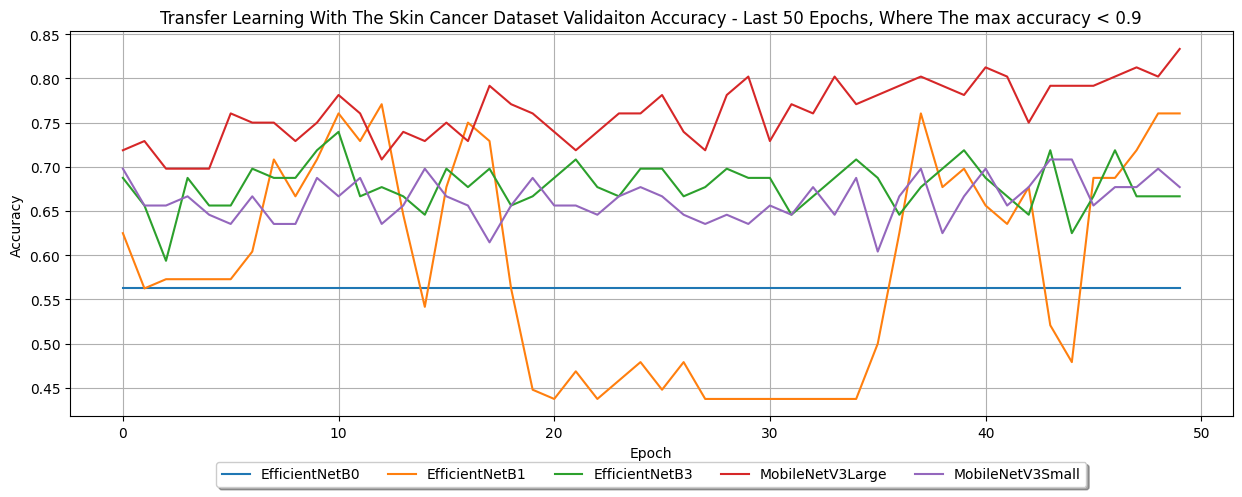
\includegraphics[width=1\textwidth]{images/Skin-cancer-validation-accuracy-last-50-low-performers.png}
\end{figure}

These models are the lower performers in the skin cancer dataset, none of them ever scored above 90\% accuracy on the validation data, they all also were clearly distinguished from the other models in their training loss. Mobilenetv3 Large has typically been a good performer with the Alzheimer's dataset, however here it's performing comparatively poorly.

The efficient net models are also performing poorly, this is likely due to the fact that the efficient net models are comparatively very small, and may not have enough capacity to effectively capture the more complex features of the skin cancer images, as opposed to classifying images of hotdogs or not hotdogs, for example. None of these models are specifically designed to classify smaller details in images, however many of them have the capacity to do so, it just may have been pruned too much for it to be effective at this task.

\begin{figure}[ht!]
  \centering
  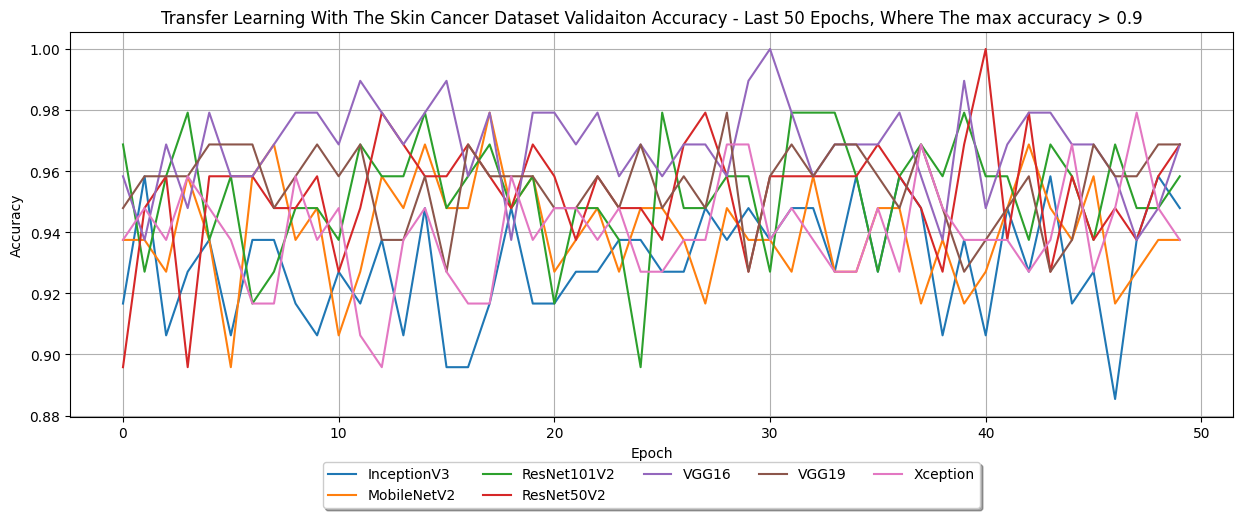
\includegraphics[width=1\textwidth]{images/Skin-cancer-validation-accuracy-last-50-high-performers.png}
\end{figure}

These models with a maximum validation accuracy of over 90\%, typically all perform very well, not dipping below the 90\% mark often. As this graph shows too, many models achived a consistent accuracy of over 96\% on the validation data, which is very good for the amount of time it took to train them. VGG16 typically performed the best with this dataset, and it's the smallest model that performed well. This could have been a coincidence, however it's undenyable that VGG16 is a very good model for this application.

\begin{figure}[ht!]
  \centering
  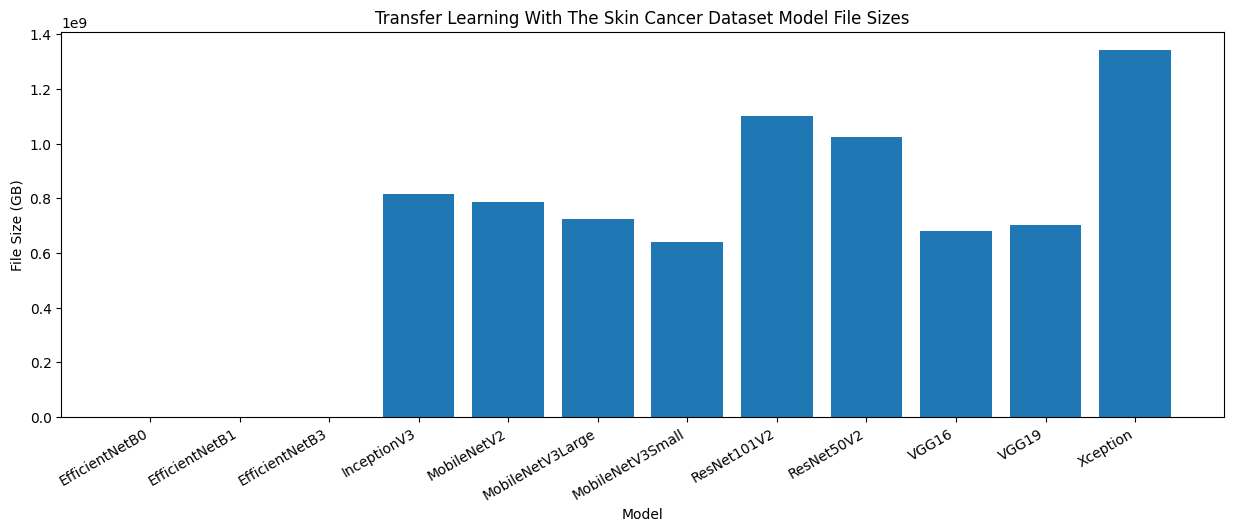
\includegraphics[width=1\textwidth]{images/skin-cancer-model-sizes-graph.png}
\end{figure}

Now that I've got the initial training results, I'm going to try and see if I can use hyperparameter optimisation, and see if I can get the models to perform even better. I'll also try adjusting the augmentation parameters and see how that affects the results.

\subsection{Optimising the EfficientNet Models}

Due to the outstanding performance of the EfficientNet models in the ImageNet challenge, I decided to try and optimise one of the best models in the series too see if I can get it to perform on the same level as the other models. For this, I have chosen to use the newer and slightly larger EfficientNetV2B1 model. For this test I have decided to not change the brightness on the validation set images as I believe that this will lead to more accurate results, better representing the real world.

I had previously done some experimenting, trying to find the best amount of layers to freeze in the model, in the initial training stages where the learning rate is higher, and for this, I had determined that freezing all the layers in the base model aside from the last 35 gave me good results to get started with.

% Show image of EfficientNetV2B1-initial-training-loss.png

\begin{figure}[ht!]
  \centering
  \begin{subfigure}{0.4\textwidth}
    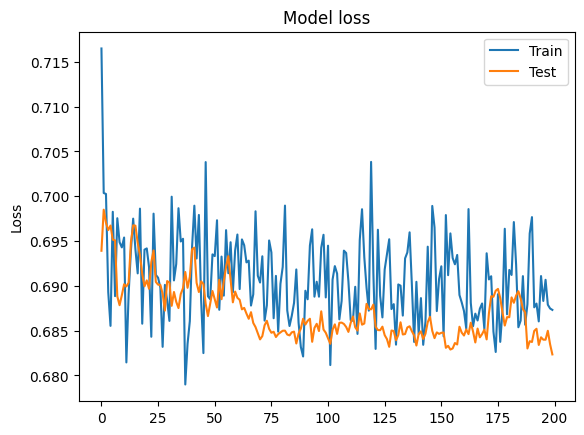
\includegraphics[width=\linewidth]{images/EfficientNetV2B1-initial-training-loss.png}
    \caption{Training Loss}
    \label{fig:EfficientNetV2B1-initial-training-loss}
  \end{subfigure}
  \begin{subfigure}{0.4\textwidth}
    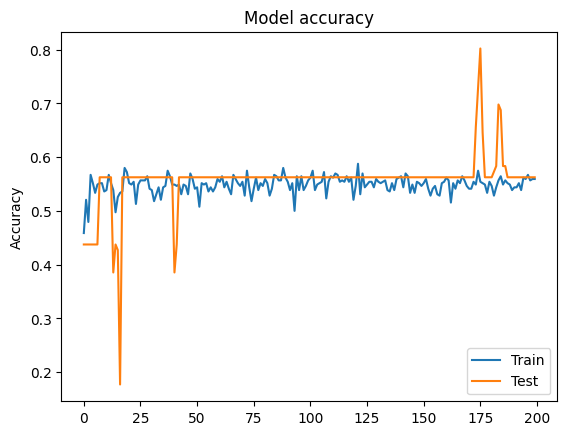
\includegraphics[width=\linewidth]{images/EfficientNetV2B1-initial-training-accuracy.png}
    \caption{Training Accuracy}
    \label{fig:EfficientNetV2B1-initial-training-accuracy}
  \end{subfigure}
  \caption{Initial Training Loss and Accuracy of EfficientNetV2B1}
  \label{fig:EfficientNetV2B1-initial-training}
\end{figure}

The first 200 epochs as shown in the figure \ref{fig:EfficientNetV2B1-initial-training-loss} shows that there is really not much progress with the training. The loss is not decreasing much at all. The accuracy graph tells the same story too, there is essentially no progress made with most of the base model's layers frozen.


\begin{figure}[ht!]
  \centering
  \begin{subfigure}{0.4\textwidth}
    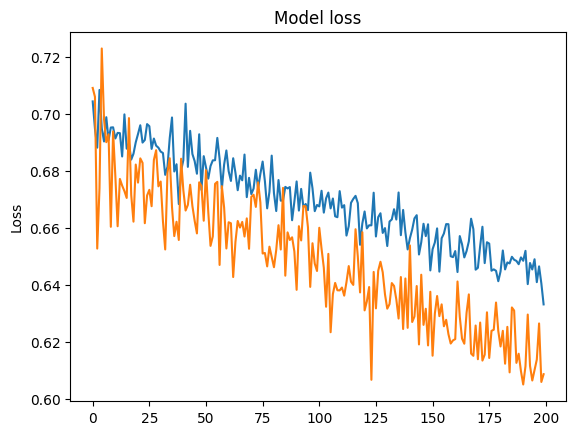
\includegraphics[width=\linewidth]{images/EfficientNetV2B1-2nd-training-loss.png}
    \caption{Training Loss}
    \label{fig:EfficientNetV2B1-2nd-training-loss}
  \end{subfigure}
  \begin{subfigure}{0.4\textwidth}
    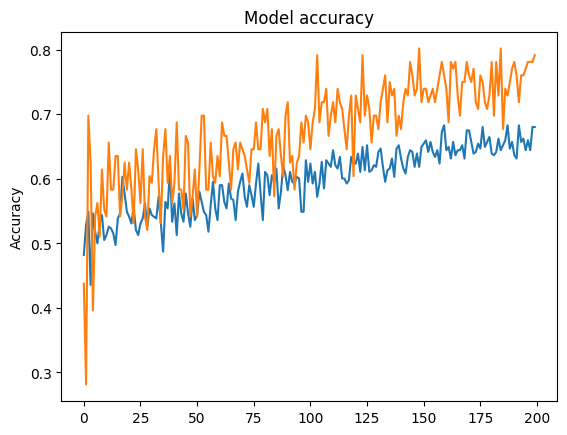
\includegraphics[width=\linewidth]{images/EfficientNetV2B1-2nd-training-accuracy.png}
    \caption{Training Accuracy}
    \label{fig:EfficientNetV2B1-2nd-training-accuracy}
  \end{subfigure}
  \caption{The 2nd Round of Training Loss and Accuracy of EfficientNetV2B1}
  \label{fig:EfficientNetV2B1-2nd-training}
\end{figure}

The progress made after unfreezing all of the base model and turning the learning rate from $1 \times 10^{-5}$ to $1 \times 10^{-7}$ as this apparently allows the model to learn better from the training data. Interestingly, after reducing the augmentation on the validation set, the model's accuracy on the validation set is consistently above the training set accuracy, which is a good sign.

This clearly shows progress in the training of the model, however it is still not as good as the other models over their first 400 epochs. 

\begin{figure}[ht!]
  \centering
  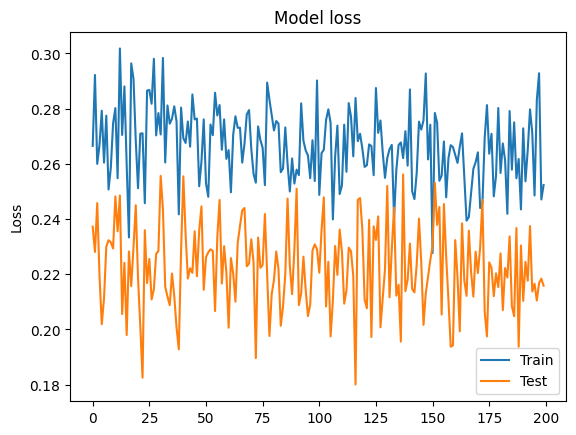
\includegraphics[width=0.7\linewidth]{images/EfficientNetV2B1-final-training-accuracy.png}
  \caption{Training Loss}
  \label{fig:EfficientNetV2B1-final-training-loss}
\end{figure}

I decided to train this model until it reaches a point where it does not appear to be improving anymore. This ended up being around 2800 epochs, which is a lot more than the other models \ref{fig:EfficientNetV2B1-final-training-loss} shows the last 200 epochs of this. This results in a final validation accuracy of 0.9375 (93.75\%) which is not as bad as it was, however it is still not as good as the other models and it took a lot longer to train to get these results.

\clearpage
After training the EfficientNetV2B1 model, as shown in the figure \ref{fig:EfficientNetV2B1-final-training-loss}, I decided to try and optimise it further through adjusting the augmentation parameters from:

\begin{lstlisting}
  train_datagen = ImageDataGenerator(
    rescale=1.0 / 255,
    width_shift_range=0.1,
    height_shift_range=0.1,
    horizontal_flip=True,
    zoom_range=0.2,
    validation_split=0.2,
    rotation_range=360,
    vertical_flip=True,
    brightness_range=(0.7, 1.3),
  )
\end{lstlisting}

to:

\begin{lstlisting}
  train_datagen = ImageDataGenerator(
    rescale=1.0 / 255,
    width_shift_range=0.2,
    height_shift_range=0.2,
    horizontal_flip=True,
    zoom_range=0.4,
    validation_split=0.2,
    rotation_range=360,
    vertical_flip=True,
    brightness_range=(0.3, 1.7),
  )
\end{lstlisting}

This was increasing the width and height shift range, increasing the zoom range, and increasing the brightness range. These augmentations were not applied to the validation set. This unfortunatley did not result in any notable improvements in the model's accuracy, as shown in the figure \ref{fig:EfficientNetV2B1-extreme-augmentation-training-loss} and \ref{fig:EfficientNetV2B1-extreme-augmentation-training-accuracy}. The model trained for 1000 epochs and the final validation accuracy was 0.9583 (95.83\%) which is slightly better than the model before I had adjusted the augmentation parameters.


\begin{figure}[ht!]
  \centering
  \begin{subfigure}{0.4\textwidth}
    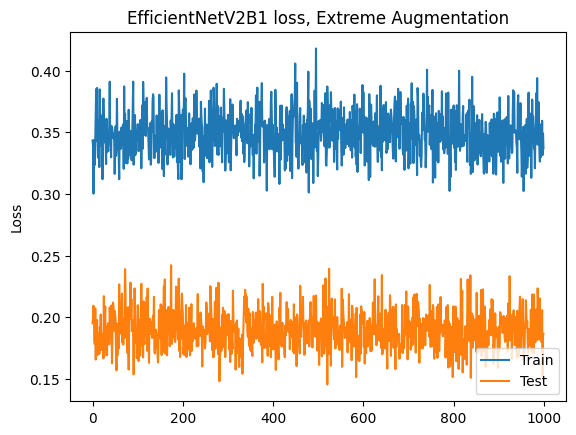
\includegraphics[width=\linewidth]{images/EfficientNetV2B1-Extreme-Augmentation-Loss.png}
    \caption{EfficientNetV2B1 Extreme Augmentation Training Loss}
    \label{fig:EfficientNetV2B1-extreme-augmentation-training-loss}
  \end{subfigure}
  \begin{subfigure}{0.4\textwidth}
    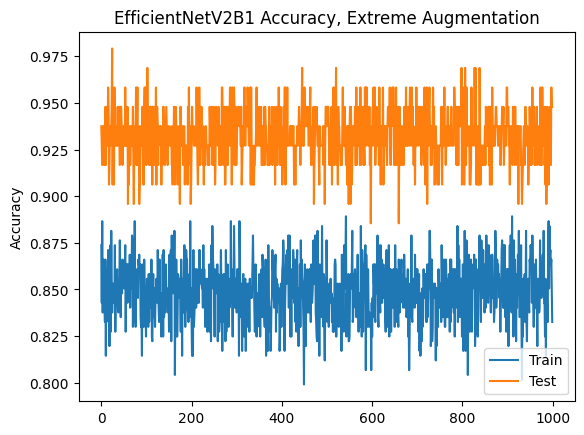
\includegraphics[width=\linewidth]{images/EfficientNetV2B1-Extreme-Augmentation-Accuracy.png}
    \caption{EfficientNetV2B1 Extreme Augmentation Training Accuracy}
    \label{fig:EfficientNetV2B1-extreme-augmentation-training-accuracy}
  \end{subfigure}
  \caption{The Extreme Augmentation Training Loss and Accuracy of EfficientNetV2B1}
  \label{fig:EfficientNetV2B1-extreme-augmentation-training}
\end{figure}

\chapter{How to run the code}

\section{The Frontend Installation and Setup}

\subsection{Installing Node.js}
To install Node.js\cite{NodeJs}, go to the Node.js website and download the latest version of Node.js for your operating system. 
Follow the instructions to install Node.js.

\subsection{Installing Yarn}
To install Yarn\cite{Yarn}, go to the Yarn website and download the latest version of Yarn for your operating system.
Follow the instructions to install Yarn.

\subsection{Installing the dependencies}
To install the dependencies for the frontend, run the following command in the frontend directory:
\begin{lstlisting}
  yarn
\end{lstlisting}

\subsection{Running the frontend}
To run the frontend, run the following command in the frontend directory:
\begin{lstlisting}
  yarn dev
\end{lstlisting}

\subsection{Building the frontend}
To build the frontend, run the following command in the frontend directory:
\begin{lstlisting}
  yarn build
\end{lstlisting}

This will create a folder under ./dist/ which contains the built frontend.

To see the code running and deployed, go to the GitHub Pages site\cite{Hosted-UI}.

\subsection{How to use the UI}

To use the UI, with the Alzheimer's Disease Classification model, or the Skin Cancer Classification model,
the UI is very simple to use and only contains very few buttons.

One aspect of the library which is not as clear, due to the library I am using, is the cropping with the skin cancer input.
The interface is designed to be mobile compatible and therefore the cropping is done by dragging your finger and closing in on the skin area that you want to analyse.
In figure \ref{fig:UI-Cropping} you can see that the cropping is not very clear all the time, so the user may need to be prompted on how to use the cropping.
This may be fine, as 

\begin{figure}[ht!]
  \centering
  \begin{subfigure}{0.4\textwidth}
    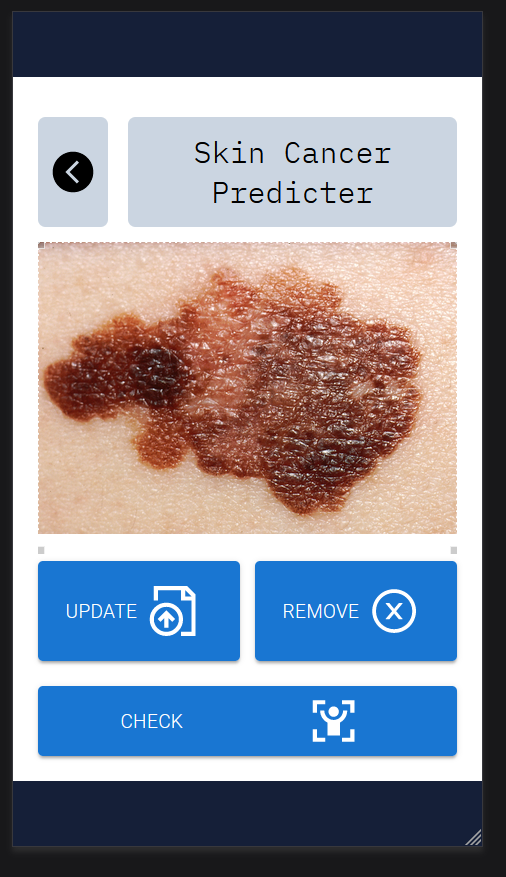
\includegraphics[width=\linewidth]{images/UI-screenshot-unclear.png}
    \label{fig:Unclear-cropping}
  \end{subfigure}
  \begin{subfigure}{0.4\textwidth}
    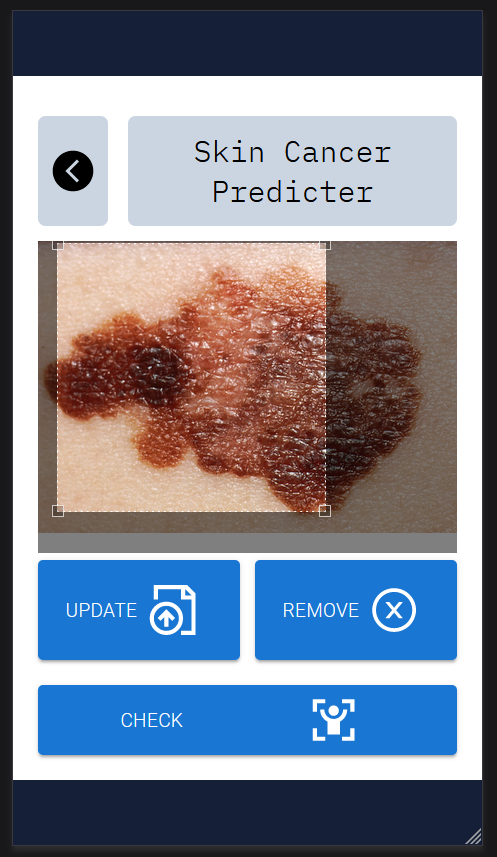
\includegraphics[width=\linewidth]{images/UI-screenshot-clear.png}
    \label{fig:Clear-Cropping}
  \end{subfigure}
  \caption{The Skin Cancer Cropping UI}
  \label{fig:UI-Cropping}
\end{figure}


\section{The Python Side of the Project}

\subsection{Prerequisites for the Python code}
Go to the directory in your powershell terminal (with python 3.7 > installed) and run the following command:
\begin{lstlisting}
  pip install -r requirements.txt
\end{lstlisting}

I believe this would run on Linux/Unix too, however I have not tested it, due to my main OS being Windows.

\subsection{Running the Notebooks}

This should install the required packages for the python side of the project.
To run the code in the notebook, follow the markdown instructions in the notebook.
To run the training program, run automated-testing-training/main.py (it will likely take a long time to run).

To run the tests for the AutomatedTestingLibary run the following command:
\begin{lstlisting}
  python -m pytest 
\end{lstlisting}
Run main.py in the AutomatedTestingLibary directory to run the training program.

\chapter{Professional Issues}

% TODO: talk about the agreements made to get the data, and the potential issues with the data

\section{Usability}
As AI-based systems such as transfer learning models are increasingly employed for Alzheimer's detection, it is crucial to ensure that they are accessible, user-friendly and transparent in their operation. The algorithms should be focused on designing systems that complement human expertise rather than replacing it, facilitating seamless integration between healthcare professionals and AI tools. Appropriate training and guidelines for the use of AI in medical imaging should be implemented to ensure that healthcare providers are comfortable and proficient with the technology. This would mean that my web interface should be intuitive and easily accessible to healthcare professionals, and should be able to be used by them without any training.

\section{Plagiarism}

To prevent unethical practices and promote collaboration, it is essential to establish guidelines for the appropriate use, citation, and acknowledgment of research materials and software. When using code or datasets from other sources, I have quoted the source and provided a link or citation to the original work.

\section{Safety and Reliability}

The validity and reliability of AI models are critical for maintaining trust in the technology, especially when dealing with sensitive healthcare data. Rigorous testing and validation methods should be employed to ensure the accuracy of the model. Furthermore, healthcare providers and patients should be made aware of any "as is" clauses or other limitations associated with the software to prevent misuse or over-reliance on the technology. As the accuracy of the models is not guaranteed, I will need to ensure that the output is clearly displayed from the model and the confidence scores for each class are also displayed, to help the healthcare professional make a decision. The models used in this project would most likely be better suited for screening patients, rather than making a final diagnosis.

\section{Privacy and Legal Issues}

The use of machine learning for Alzheimer's diagnosis raises significant privacy concerns, particularly with regard to the handling and storage of sensitive patient data. Data protection laws and regulations, such as HIPAA and GDPR, must be adhered to in order to guarantee patient confidentiality and to secure informed consent for the collection of medical data. Data anonymization techniques should be used to protect patients' identities when training and utilizing AI models. For the OASIS datasets, the data is already anonymized, but there are also other terms and conditions that must be followed, for example, with MRI scans, you can generate an image of the patient's face and use that to identify the patient and that was explicitly forbidden in the terms and conditions.

Machine learning is also used in other areas of healthcare, such as drug discovery and clinical trials, for example, a drug may get killed off in it's early stages if an algorithm determines that it could be carcinogenic. This could be a problem if the algorithm is wrong, as the drug could have been a significant breakthrough treatment, however it's likely to have a better impact to use the prediction algorithm to screen drugs and get the problematic ones removed quicker, as more resources can be put into the drugs that are more likely to be successful.\cite{10.3389/frai.2021.757780}

\section{Monopoly and Competition}

The AI healthcare market should remain competitive and accessible to various stakeholders, preventing the dominance of a few companies or technologies. The avoidance of proprietary formats, DRM measures, and forced tie-ins is crucial for maintaining a fair marketplace and providing healthcare professionals with multiple options for AI-assisted Alzheimer's diagnosis and treatment. Specifically, the BIDS format should be used to store and interpret the data, as it is an open standard for neuroimaging data. In terms of competition, Keras, Tensorflow and the pre-trained models are all open source, so anyone can use them, and there are many other open source libraries that can be used by anyone, so the competition is not a huge issue.

\section{Management and Stakeholder Consultation}

There are various stakeholders who would be interested in AI prediction of Alzheimer's, for example the patients could be interested in knowing if they have Alzheimer's quicker than they otherwise would have, however the patients having direct access to the web interface would be problematic, as the results may be inaccurate and could potentially cause un-needed stress for the patient.

The healthcare professionals would be interested in the web interface, as it would allow them to quickly and easily get a prediction of whether the patient has Alzheimer's or not, and it would also allow them to see the confidence scores for each class, so they can make a more informed decision, this interface being available 24/7 and being easy to use would benefit them greatly. The usability to the healthcare professionals would depend on the accuracy of the model too, so it would be important to ensure that the model is as accurate as possible.

\section{Biases in the data}

The biases in the OASIS-1 dataset are very prevalent, I have decided to dedicate a seperate chapter to this issue. Giving the machine learning model the age of the patient as a feature could potentially be a bad idea, as the biases in the data could potentially lead to the model predicting whether or not the patient has AD, based off of their age. If I don't give the model the age of the patient, there is a chance that it could predict the age it's self, which would defeat the purpose of the model. I could try predicting the age of the patient to see how well it can guess the age of a patient based off of their MRI scan, to see if it has the ability to predict the age of the patient, I could also see how changing the given age of the patient affects the accuracy of the model, accross the different classes.

\section{Collaboration and Communication Barriers}
If the model's accuracy is not explicitly stated in the web interface, doctors may be more likely to rely on the models predictions, rather than using their own judgement, which could lead to a misdiagnosis. The model's accuracy should be clearly stated in the web interface, so that the healthcare professionals can make an informed decision, and the interface should have a disclaimer stating that the model's accuracy is not guaranteed, and that the healthcare professional should use their own judgement when making a diagnosis, along with multilingual support, so that the interface can be used by healthcare professionals from all over the world, without any potential problems with language barriers.

\section{Bias in the Skin Cancer Dataset}
The skin cancer dataset has a variety of different photos of benign and malignant blemishes on skin, however all of the images are of caucasian people, with there appearing to be no variety in terms of skin colour. This means that this model would only benefit anyone of caucasian descent, and it would not be reliable with any other skin colour. This is a problem as the dataset is not representative of the world's population, which could lead to non-caucasian people getting a lower quality of healthcare, as they would not be able to use the model to get a diagnosis of their skin cancer.
On the other hand, prediction of skin cancer would be a lot more accurate for caucasian people as opposed to people with darker skin, as the melanin in their skin would make it harder to see the blemishes and make out what they are. This specific problem would be beyond the scope of this report, however it would be something to consider for anyone using this dataset for other projects.

\section{Data Privacy and Security}
Data privacy and security for any medical data is a huge issue, and it is important to ensure that the data is secure and that any patients who use their data with my user interface. This was part of my decision to have all the data processing locally on the user's computer, as it would mean that the data would not be sent to any servers, and it would also mean that the data would not need to be stored on any servers either. This would avoid all medical data handling regulatory issues from legal bodies/statutes such as HIPAA and GDPR, which require extremely strict data handling procedures to be followed, which takes a lot of time and effort to implement, and it would also avoid any potential legal issues that could arise from not following the regulations. This is the best solution for a project like this as the models are only around 40MB max for some of the good models I have tried, so it wouldn't take longer than a few minutes at most to download the model. Another potential drawback is the model might be too large for devices with low processing power to run, however modern phones are very powerful and have GPU acceleration which the library the models use online can take advantage of.

\chapter{Diary}

\section*{19/10/2022}

Today I have been deciding the specific classes of images I want to use for my project.
I had initially intended on using only 1 class, however I have decided to use 2 classes instead as I think it will be more interesting to see the results of the transfer learning on 2 classes rather than 1,
It will also demonstrate better the different strengths and weaknesses of the individual transfer learning methods.

I have decided to use the following sets of images:

% List the datasets
\begin{itemize}
  \item \href{https://storage.googleapis.com/download.tensorflow.org/example_images/flower_photos.tgz}{Flowers Dataset}
        This dataset is likely to be an easier dataset for the models to get high accuracy on, as the different flowers are quite distinct from each other.
  \item  \href{https://www.kaggle.com/datasets/uraninjo/augmented-alzheimer-mri-dataset}{Alzheimer's Dataset}
        This dataset is going to be more difficult for the models as the changes are more subtle between the different scan images, and the images are not as distinct from each other.
\end{itemize}



I am going to follow the tutorial \href{https://www.tensorflow.org/tutorials/images/classification}{here}
which should help me to get a good understanding of how to use the datasets and how to train the models to start with.
I have no prior experience training models so this will be a good starting point for me.
I will then need to use parts of the code from the tutorial to transfer run the transfer learning.

\section*{26/10/2022}


Today I have been working on the transfer learning tutorial, I've made more progress through it and I've managed to get
Mobilenetv3 to run on the flowers dataset, however I'm having some issues with the alzheimer's dataset.
This is significant progress as this was a major blocker for me as I was not sure how to go forward with the prediction.

\section*{01/11/2022}

Today I've worked more on the transfer learning tutorial and it can now identify the different flowers in the flowers dataset,
with varying degrees of accuracy, around 80\% was the best I got however this was only after 5 epochs and was the first time I have tried transfer learning.

\section*{09/11/2022}


I had lost some of my git history for my diary, so I have had to rewrite some diary entries.
I have found more flower dataset images here and I've decided to change over to this as soon as possible;
\href{https://www.kaggle.com/competitions/tpu-getting-started/overview}{https://www.kaggle.com/competitions/tpu-getting-started/overview}

\section*{14/11/2022}

I am training the model "Mobilenetv3 Small" with the Alzheimer's dataset, I have been able to get it to run and it is currently training.
The power required to train the models is making it difficult to use trial and error for the parameters, so I am going to try and find a way to use the GPU on my laptop to train the models as soon as possible.
I'm also going to optimise the way I am training the models as to not use more power than necessary. This means I've got to get a better understanding of the models I am training with and how they work.
I have found this paper Searching For MobileNetV3\cite{DBLP:journals/corr/abs-1905-02244} which I think will be useful for me to read through and understand the structure of Mobilenetv3.

\section*{15/11/2022}

I've had trouble getting the Alzheimer's classification to work with transfer learning, so I decided to try and run other people's code to see if I could get it to work.
I have found that my transfer learning could be significantly more efficient and accurate if I use the existing code, so I'll have to try and identify where I went wrong with my code and make improvements.

\section*{21/11/2022}

Today I managed to get the accuracy up to 90\% on the alzheimer's dataset, this is a significant improvement from the 60\% I was getting before. My model appears to still be overfitting however this progress is good. This was done through transfer learning on the Mobilenetv3 small model.

Output from the model during fine-tuning:
\begin{lstlisting}
  loss: 0.0314 - accuracy: 0.9883 - val_loss: 0.1337 - val_accuracy: 0.9036
\end{lstlisting}

\section*{22/11/2022}

Here's some graphs of the model's predictions on the alzheimer's dataset:
This graph was made using the MobilenetV3Small model and transfer learning on the Alzheimer's dataset, with all but 3 layers of the mobilenetv3 model frozen.
![image](/images/better-output.png)
% convert markdown to latex
\begin{figure}[ht!]
  \centering
  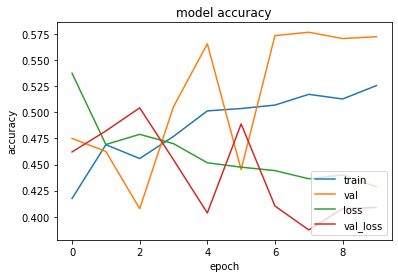
\includegraphics[width=0.8\textwidth]{images/better-output.png}
  \caption{Graph of the model's predictions on the alzheimer's dataset}
\end{figure}

\begin{figure}[ht!]
  \centering
  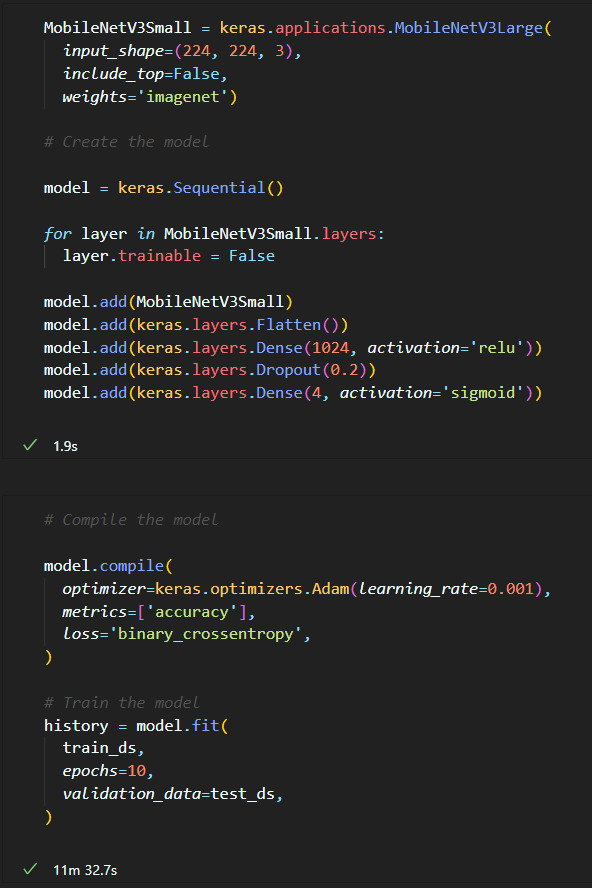
\includegraphics[width=0.8\textwidth]{images/training.png}
  \caption{Code used to generate the graph}
\end{figure}

\begin{figure}[ht!]
  \centering
  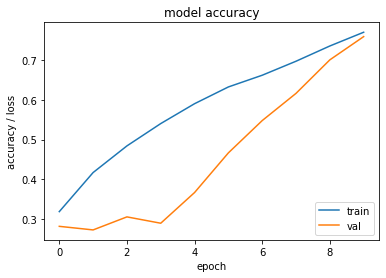
\includegraphics[width=0.8\textwidth]{images/positive-progress.png}
  \caption{Positive progress from unfreezing all the layers of the model and "fine-tuning" the model}
\end{figure}

Here is a graph of where I was fine-tuning the model however I had overfitted the model and it was not generalising well to the test data:

\begin{figure}[ht!]
  \centering
  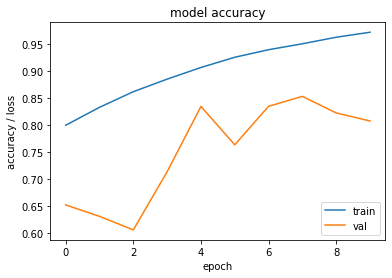
\includegraphics[width=0.8\textwidth]{images/fine-tuning-more.png}
  \caption{Graph of where I was fine-tuning the model however I had overfitted the model and it was not generalising well to the test data}
\end{figure}

![image](./images/maxing-out.png)
% convert markdown to latex
\begin{figure}[ht!]
  \centering
  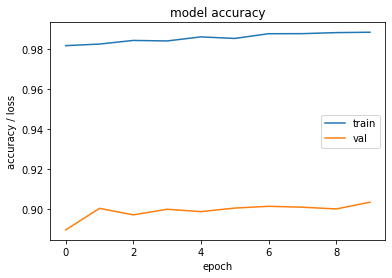
\includegraphics[width=0.8\textwidth]{images/maxing-out.png}
\end{figure}


\begin{figure}[ht!]
  \centering
  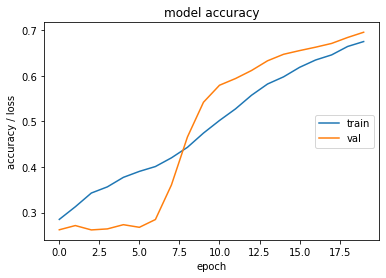
\includegraphics[width=0.8\textwidth]{images/mobilenetv3-first-attempt.png}
  \caption{First attempt at training the mobilenetV3Large model after unfreezing all the layers}
\end{figure}

I have also setup my laptop properly using Manjaro Linux to train the models on the GPU, this should make it much easier to train the models and to try different parameters and should allow me to create a confusion matrix for different parameters.

\section*{23/11/2022}

I have achieved 99\% accuracy on my model identifying Alzheimer's (validation dataset). This was unfortunatley not saved however as it crashed, however I believe I can get it to that level again.
I have written a scritpt to use different base models for transfer learning and to output the results of training to a JSON file, so I can analyse the results later, it also saves the model to a file, so I can use it later.
This should make it a lot easier to use different models, datasets and parameters to train the models and to analyze the results and make the confusion matrix.

\section*{27/11/2022}
I have been working lots on the interim report and getting it ready to submit, during this time I have also been setting my laptop off to train the models
as I work. I discovered that my '99\%' accuracy was from the model learning the validation set through the augmented images, so I have had to retrain all the
models with images I have augmented myself.

Soon I'll finish the Alzheimer's dataset training, and I'll start working on the flower's dataset.

\section*{28/11/2022}

Today I have had trouble with the training, my GPU kept running out of memory due to me not releasing the ram after the keras model was trained. This meant I had to keep on checking and restarting the training, every few models. This is now fixed, and I have been able to train the models without any issues. They are currently training and there is a lot of progress to be made.

\section*{29/11/2022}

Today I have decided to start work on the training and testing library which I can use to speed up training and increase reliability of my training, through unit tests and consistency.
This library will allow me to adjust parameters for fitting and compilation to let me easily do hyperparameter tuning.

\section*{1/12/2022}

I have been working lots on my report and the training library, this has taken a while to get all the information I feel I need in my report, however I have now mostly finished it and will submit it soon.

I have made lots of graphs from the history of the models in training, this made it a lot easier to talk about the different strengths and weaknesses of the different base models.

\section*{24/1/2023}
I've manually reviewed my dataset I'm using, and I've found it to have multiple repeated images. Due to the poor quality of the dataset I'm using I've decided to use a different dataset for my project, which I believe is the original data from the corrupted dataset I was using.
https://www.oasis-brains.org/

This dataset has more information about the patients, such as their sex, age and different scores on tests relating to the disease.

This also allows me to predict whether or not a person has Alzheimer's from all the MRI scans they have taken, rather than just one.

I hope to get this dataset working soon and to start training the models, and I'm aiming for at least a 90\% accuracy on the validation dataset.

\section*{15/2/2023}

I've downloaded the OASIS dataset 1 and I've created some graphs to analyze the data and to try and identify potential biases in the data. The main problem with it is that there are few MRI scans of people with Alzheimer's, and they're mostly old, which means if the model is given the age of the patient, it will cause bias with it, as it's more likely to be an older person with Alzheimer's in this dataset. I need to identify what different parameters given alongside the MRI scans in the dataset will cause bias with the model (primarily by giving the model the age of the patient).

\section*{28/2/2023}

I have decided to create a web-UI for my project, this will allow me to easily show the results of the models and to allow people to upload their own images to test the models on. This should be easy to do with Flask and I hope to have it done soon.

I've also started downloading the new OASIS dataset again after I ran out of space on my hard drive.

\section*{5/3/2023}

I've purchased an RTX 3080 to help speed up my training and to allow me to train larger models. After installing this hardware, my training times have been significantly reduced, and I have 2 GB more v-ram to use.

\section*{10/3/2023}

I have managed to get the OASIS-1 dataset training with transfer learning, as its format is different to the dataset I was previously using (it's a collection of files, rather than 4 folders with the different categories of images in them). This was done through the Pandas library, using the dataframe class, along with the keras ImageDataGenerator class which helps me read the images from the dataset, along with batching them to be used in training (so my GPU doesn't run out of memory), as well as augmenting the images to help prevent overfitting.

The performance of the model on the new dataset however is significantly lower than I would like. The previous dataset gave me false hope, as the repeated images were in the training and validation classes, giving me a far higher accuracy than I actually had. I will experiment with hyperparameter tuning and I will look into using the other information in the OASIS-1 dataset to help improve the accuracy of the model, as features in the OASIS model include
```
ID,M/F,Hand,Age,Educ,SES,MMSE,CDR,eTIV,nWBV,ASF,Delay
```

During this time, I've also managed to get ill, so I haven't been able to work on the project as much as I would like.

\section*{14/3/2023}

To use the seperate parameters, alongside the MRI scans, I will need to create a custom model, which will take in the parameters, then I will also use the original transfer learning model, and combine the outputs of the two models to create a new model. This will allow me to use the parameters and the MRI scans, which will hopefully improve the accuracy of the model.

Combining the models will be done through the Keras Model class, which allows me to create a new model from the outputs of other models, however I am struggling to pass the data to the new model, as I have had many errors when trying to pass the new data and the MRI scans to the model. I will continue to try and fix this issue today.

\section*{15/3/2023}

I have had many problems combining the age, gender and other information about the patients with the MRI scans, the problem lies with the fit function of the model as the method I was using to get the images from the dataset originally, did not allow for other data to be included as an input for the model. I have now created my own generator class and intend to use that to get the data from the dataset and pass it to the model.

\section*{16/3/2023}

After lots of struggling, I have managed to get my custom generator working with keras, it now trains and has the MMSE, age and gender as context. I'm still having trouble with the accuracy but hopefully with more parameters, it will improve.

I've also encountered a problem with the training, as the validation accuracy is almost always 0.9195, and this doesn't seem to change much. I will try adjusting the training/validation split to see if anything improves.

\section*{19/3/2023}

I have continued to work on the report today, and I've got most of the web-ui working now, I just need to display the results of the models on the web page. I have begun to go through the markscheme and add sections such as the professional issues to my report, along with Rationale.

\section*{20/3/2023}

I've merged the git branches into main, as I wanted to ensure I do not have too many conflicts closer to the deadline, and to ensure that I will not lose work due to a merge conflict.

I have also decided today to not use the OASIS-3 dataset, as it's not as well documented as the OASIS-1 dataset, and the different scan formats are not easily passed to the model. The OASIS-1 dataset has preprocessed images which are easier to use and train with, whereas the raw OASIS-3 scans would most likely require a different model structure to be used (such as an LSTM, which is not typically used).

Today I will try and get the basic transfer learning results finished and save them to a file, so I can use them in the web-ui.
The web-ui is mostly finished now, I just need to add the results of the models to the web page.

I have managed to get the basic transfer learning results saved to files, along with the training and loss results.

\section*{21/3/2023}

Today I've been working on my report, adding different sections on the Alzheimer's disease, and why it's so important to diagnose it early.

\section*{22/3/2023}

I've been working more on the report and getting the web-ui working, I've battled with CORS to get the POST request through to flask and I've managed to get the majority of it working.

\section*{23/3/2023}

I have decided to get the training results for all the different models with the Alzheimer's dataset, and save them to files, so I can use them in the web-ui. The performance of these models is not great, so I will have to find ways to make this better.


\section*{24/3/2023}

Today I have been given a skin cancer dataset to use for my project, I will be using this to train a model to classify benign and malignant blemishes on the skin. I will be using transfer learning to train the model, and I will be using the same model structure as I used for the Alzheimers dataset.

The results from training these models has been very positive, and I have managed to get a consistent accuracy of 0.98 on the validation set, which is very good. I will continue to train the model and see if I can get the accuracy any higher.

\section*{25/3/2023}

Today I have created graphs from the different training results with the skin cancer dataset, I will use these to talk about the performance of the different models in my report. 

\section*{26/3/2023}

I have been working more on my report, as I have my graphs to analyze and talk about in the report. I am going to try and increase the accuracy of the EfficientNet models and potentially use the newer EfficientNetV2 models to try and boost performance.

\section*{27/3/2023}

Today I want to try and optimise the EfficientNetv2 models more and do a write-up on the results for them, then I will try and use hyperparameter tuning to try and improve the performance of the better performing models to see how high I can get the accuracy.

I also want to try to get the web-ui working with the server side processing, so I can get the results of the models on the web page and then I want to experiment with tensorflow-JS to see if I can get the models to run in the browser for increased privacy and lower running costs.

\section*{28/3/2023}

Today I have been training more models to try and optimise the performance of them in the Alzheimer's dataset.

I've also got the web-ui working with the client side processing, so I can give the user the results of their images locally, which avoids the need for the server to process the images. There are many advantages to this, one of which is that I can deploy to a static file hosting service, such as GitHub pages, which means I can indefinitely host the web-ui for free.

I will continue to refactor the server side code to submit it to my project code, however I will not use it.

\section*{29/3/2023}

Today I will be working on my report, ensuring there are no spelling mistakes, repeated sections and that the report is well written and easy to understand.
I have also been working on the web-ui, and I have managed to get the results of the models to display on the web page.

\section*{30/3/2023}

Today I've been refactoring my code and report to ensure it's in the best possible state it can be in, I've also been working on the web-ui, and I have managed to get the results of the models to display on the web page.
The web-ui now works and is hosted on github pages, this is on my GitHub page and can be found here\cite{Hosted-UI}.

\chapter{Conclusion}

This project has been a huge learning experience for me, I had never trained, optimised or deployed a machine learning model before, and I have learned a lot about the process of doing so. I have also learned a lot about the cutting edge image classification techniques, including transfer learning. I have also learned a lot about how hyperoptimisation works and how to use it to improve the performance of a model.

I have also learned a lot about the Alzheimer's disease, and how important it is to diagnose it early, as it can have a huge impact on the quality of life of the patient. I have also learned a lot about the different types of scans that are used to diagnose Alzheimer's, and how they can be used to detect the disease. 

Although my results from the Alzheimer's dataset were not as good as I would have liked, I have still learned a lot from this project and I am very happy with the results from the skin cancer dataset, as I was able to get a very high accuracy on the validation set.

\section{Challanges and how I overcame them}

I had many problems with the Alzheimer's dataset, however after learning how to use the OASIS-1 dataset, I was able to get some better and more reliable results. I realise how it would have been much better if I were to go straight to the OASIS-1 dataset, however I was not aware of it until I was already deep into the project. Luckily I was able to get some good results from the skin cancer dataset, and I was able to use these results to talk about the performance of the different models in my report.

I had spend many hours trying to find out how to parse batches of images and floats together into a model, to try and increase the accuracy that I got on the OASIS-1 dataset. I eventually found out that I had to use a custom data generator, which I was able to use to parse the images and floats together into a model. I was able to get a much better accuracy from this, and with some of the models I tried to optimise the performance of, I was able to get a consistent accuracy of \%95.83 on the validation set with EfficientNetV2B1 or 97\% with VGG19.

I have also had some few problems with TensorflowJS\cite{smilkov2019tensorflowjs}, as I was not able to get all the models to run in the browser as not all of the keras layers have been implemented in the JS library. The `Normalisation` layer was not implemented, so I had to remove that model from the web-ui. This was not a huge deal as I was able to get the other models to run in the browser, and I was able to get the results of the models on the web page.

\section{Future Improvements I Could Make}

I could try and dive deeper into the EfficientNetv2 models and see if they would perform better than the other models, as their performance on the ImageNet\cite{ImageNet} dataset was very good. 

I could also try and parse the raw MRI information into the model, as I was not able to do this due to time constraints. This could potentially make my model more accurate and it would at least be interesting to see if it could make a difference, as I would have to give a model a 3d input, instead of just 2D. I'd have to see if I could use the BIDS data format to parse the raw MRI data into the model, I could also think of ways to pre-process the data to make it easier to parse into the model, as well as augmenting the data to make the model more robust. Part of the reason for me not doing this was because that I could not have used transfer learning to train the model, as I would have had to train the model from scratch, which would have taken a lot longer and not been the objective of this project.

Other improvements could be to expand the web-ui to include more models and potentially combine some of the models outputs to get a more accurate result. This would need to be done with caution, as I would have to make sure that the models are not too similar and I would likely have to prune the models to get the best results.

I would also like to take a look into pruning the models I have trained, all of the base models I have used for transfer learning have been trained on the ImageNet dataset, which is a very large dataset, and I would like to see if I can get the models to run faster by pruning them and potentially removing lots of un-nessasary nodes or layers from the model. The Lottery ticket hypothesis\cite{LotteryTicket} could be used to find 'winning tickets' in the models, which are the smallest subnetworks that can achieve the same accuracy as the original model.

\section{The Main Things I Have Learned}

I learned how to pre-process data through augmentation and normalisation, and how to use transfer learning to train a model. I have also learnt how to use TensorFlowJS to create a client side web application, which can be deployed to a static file hosting service, to allow anyone with an internet connection and modern hardware to quickly and easily use any most of the models I have trained.

I have also learned about the cutting edge image classification models and techniques that are being used in the industry today and how they work, and what improvements they have made over the years.

\newpage
\printbibliography
\label{endpage}

\end{document}
\end{article}